\documentclass{article}

\usepackage{coursenotes}

\set{AuthorName}{TC Fraser}
\set{Email}{tcfraser@tcfraser.com}
\set{Website}{www.tcfraser.com}
\set{ClassName}{Quantum Physics 3}
\set{School}{University of Waterloo}
\set{CourseCode}{Phys 434}
\set{InstructorName}{Anton Burkov}
\set{Term}{Fall 2016}
\set{Version}{1.0}

\draftprofile[TC Fraser]{TC}{Purple}

\newcommand{\hilb}{\mathcal{H}}

\begin{document}

\titlePage

\tableOfContents

\disclaimer

\section{Review}

\subsection{Discrete Spectrum}
States in quantum mechanics are vectors in Hilbert space $\hilb$. In Dirac notation, states are denoted as \textit{kets} $\ket{\psi}$. Observables in quantum mechanics are operators $A : \hilb \to \hilb$ such that $\ket{\psi} \mapsto A \ket{\psi}$. Every operator $A$ has a set of eigenkets $\bc{\ket{a'}}$,
\[ A \ket{a'} = a' \ket{a'} \]
The eigenvalue corresponding to the eigenket $\ket{a'}$ is denoted $a' \in \R$. \\

The dual Hilbert space will be called the bra space and elements of the bra space will be denoted with a bra $\bra{\varphi}$.\\

We will denoted the \textit{inner product} (scalar product) to be $\braket{\varphi}{\psi}$. By definition,
\[ \braket{\varphi}{\psi} = \braket{\psi}{\varphi}^{*} \]
\[ \braket{\psi}{\psi} = \norm{\psi} \geq 0 \]

Every state in the Hilbert space can be normalized,
\[ \ket{\ti{\psi}} = \f{1}{\sqrt{\braket{\psi}{\psi}}} \ket{\psi} \]

In doing so, we have,
\[ \braket{\ti{\psi}}{\ti{\psi}} = \f{\braket{\psi}{\psi}}{\braket{\psi}{\psi}} = 1 \]

Evidently, if we have that $\braket{\varphi}{\psi} = \braket{\psi}{\varphi}$, then $\braket{\varphi}{\psi}$ must be real. A bra $\bra{\varphi}$ and ket $\ket{\psi}$ are said to the \textit{orthogonal} if $\braket{\varphi}{\psi} = 0$. \\

The dual of $A \ket{\psi}$ is $\bra{\psi} A^\dagger$. Where $A^{\dagger}$ is the Hermitian conjugate (adjoint) of $A$. We can act on the ket $A\ket{\psi}$ with the bra $\bra{\varphi}$ and obtain,
\[ \bramidket{\varphi}{A}{\psi} = \bramidket{\psi}{A^\dagger}{\varphi}^{*} \]

The operator $A$ is \textit{Hermitian} if and only if $A = A^{\dagger}$. \\

If $A$ is a Hermitian operator, then $A$'s eigenvalues and eigenkets have particularly nice properties. Let $\br{a', \ket{a'}}$ and $\br{a'', \ket{a''}}$ be two eigen-pairs.
\[ A \ket{a'} = a' \ket{a'} \eq \label{eq:review_eig1}\]
\[ A \ket{a''} = a' \ket{a''} \eq \label{eq:review_eig2} \]
Let $\bra{\varphi}$ be an arbitrary bra. By \cref{eq:review_eig2} be have that,
\[ \bramidket{\varphi}{A}{a''} = a'' \braket{\varphi}{a''} \]
The adjoint to this equation yields,
\[ \bramidket{a''}{A}{\varphi}^{*} = a'' \braket{a''}{\varphi}^{*} \]
Conjugating each term,
\[ \bramidket{a''}{A}{\varphi} = a''^{*} \braket{a''}{\varphi} \eq \label{eq:review_gen_varphi}\]
Since \cref{eq:review_gen_varphi} is true for an arbitrary $\bra{\varphi}$, it must be that
\[ \bra{a''}A = a''^{*} \bra{a''} \eq \label{eq:review_gen_varphi_dropped} \]
Combining \cref{eq:review_gen_varphi_dropped,eq:review_eig1}, and recognizing that $A$ is Hermitian,
\[ \underbrace{\bramidket{a''}{A}{a'} - \bramidket{a''}{A^\dagger}{a'}}_{0} = a' \braket{a''}{a'} - a''^{*} \braket{a''}{a'} \]
Therefore,
\[ \br{a' - a''^{*}}\braket{a''}{a'} = 0 \eq \label{eq:review_aa}\]
As an example, we can chose $\ket{a''} = \ket{a'}$ to see that
\[ \br{a' - a'^{*}}\braket{a'}{a'} = 0 \implies a' = a'^{*}\]
Therefore all eigenvalues of Hermitian operators are always real. Since the spectrum of an operator represents all physical observables, this observation is in agreement with the fact that all physical quantities are real-valued. \\

Moreover returning to \cref{eq:review_aa} we can consider $\ket{a'}$ and $\ket{a''}$ to be different eigenkets that are non-degenerate (their eigenvalues differ). Then be \cref{eq:review_aa},
\[ \braket{a''}{a'} = 0 \]
Therefore eigenkets of Hermitian operators are orthogonal (or can at least be orthogonalized). Since the norm of an eigenket is arbitrary, we will hence forth assert that all eigenkets are normalized. Each of these properties can be summarized with a Kronecker delta.
\[ \braket{a}{a'} = \de_{a, a'} \eq \label{eq:orthonormality_discrete}\]
In summary, the set of eigenkets of any Hermitian operator forms a complete orthonormal set of states. Effectively, the set of eigenkets form a basis for the Hilbert space. Consequently, we can write any ket $\ket{\psi}$ in terms of the eigenkets for any Hermitian operator $A$
\[ \ket{\psi} = \sum_{a'} C_{a'} \ket{a'} \eq \label{eq:complete_basis}\]
Where $C_{a'} \in \C$ are uniquely defined through acting with the dual eigenket $\bra{a''}$,
\[ \braket{a''}{\psi} = \sum_{a'} C_{a'} \braket{a''}{a'} = \sum_{a'} C_{a'} \de_{a'', a'} = C_{a''} \implies C_{a'} = \braket{a'}{\psi} \eq \label{eq:coeff_determine}\]
Physically, the coefficient $C_{a'}$ is called a \textit{probability amplitude}. When a given system is in state $\ket{\psi}$, the probability of measuring the value $a'$ when making the observation or measurement $A$ is given by the square modulus of $C_{a'}$,
\[ P_{A}\br{a'} = \abs{\braket{a'}{\psi}}^2 \]
We now have the luxury of re-writing \cref{eq:complete_basis} as a spectral decomposition,
\[ \ket{\psi} = \sum_{a'} \ket{a'} \braket{a'}{\psi} \eq \label{eq:spectral_decomp_ket} \]
Since $\ket{\psi}$ is \textit{arbitrary}, we obtain a closure relation (otherwise known as the resolution of identity).
\[ \sum_{a'} \ket{a'} \bra{a'} = \ident \eq \label{eq:closure} \]
We define the projection operator $\Lambda_{a'} = \ket{a'}\bra{a'}$.
\[ \La_{a''}\ket{\psi} = \ket{a''}\braket{a''}{\psi} = \sum_{a'} \ket{a'}\underbrace{\braket{a'}{a''}}_{\de_{a', a''}}\braket{a''}{\psi} = \braket{a''}{\psi}\ket{a''} \]
As such, $\La_{a}$ \textit{projects} $\ket{\psi}$ into the direction of $\ket{a}$. Using the closure operation \cref{eq:closure} and the spectral decomposition of a ket \cref{eq:spectral_decomp_ket} one can recover the spectral decomposition of an operator $A$. For each eigenket $\ket{a'}$, multiply \cref{eq:review_eig1} by $\bra{a'}$,
\[ A \ket{a'} \bra{a'} = a' \ket{a'} \bra{a'} \]
And summing over all eigenkets,
\[ A = \sum_{a'} a' \ket{a'}\bra{a'} \]
Additionally consider another operator $B$,
\[ B = \ident \cdot B \cdot \ident = \sum_{a', a''} \ket{a''}\bramidket{a''}{B}{a'}\bra{a'} \]
Where $\bramidket{a''}{B}{a'}$ can be interpreted as a matrix indexed by $\ket{a''}$ and $\ket{a'}$,
\[ \bramidket{a''}{B}{a'} = B_{a'', a'} \]
Where refer to $B_{a'', a'}$ as the matrix elements of an operator $B$ with respect to the a complete orthonormal set of eigenstates of a Hermitian operator $A$. The entries in $B_{a'', a'}$ have the following property,
\[ \bramidket{a''}{B}{a'} = \bramidket{a'}{B^{\dagger}}{a''}^{*} \]
Therefore the matrix that corresponds to $B^{\dagger}$ is the complex conjugate transposed of the matrix corresponding to $B$.\\

\subsection{Continuous Spectrum}
Of course, there exists operators with non-discrete spectrum. We will now generalize to operators with continuous spectrum. The two most important of such operators are position and momentum. Let $\ket{\ve{x}'}$ a position eigenket corresponding to the state of a particle at position $\ve{x}'$ in space. Let $\ve{x}$ be the position \textit{operator} defined as,
\[ \ve{x} \ket{\vx'} = \vx' \ket{\vx'} \]
It is important not to get confused about notation:
\begin{itemize}
    \item $\vx$ -- Position operator
    \item $\vx'$ -- Position eigenket
\end{itemize}
The wave function $\psi\br{\vx'}$ is the probability amplitude to find a particle in a state $\ket{\psi}$ at position $\vx'$ and is defined as,
\[ \braket{\vx'}{\psi} = \psi\br{\vx'} \]
We also have the ability to generalize \cref{eq:orthonormality_discrete} to a continuous spectrum. The continuous generalization of the Kronecker delta is the Dirac delta function.
\[ \braket{\vx'}{\vx''} = \de\br{\vx' - \vx''} \]
Where $\de\br{\vx'}$ is defined as,
\[ \int_{\R^3} \dif^3 x' f\br{\vx'} \de\br{\vx'} = f\br{\ve{0}} \]
Where $f\br{\vx'} : \R^3 \to \R$ is a function on $\R^3$. \\

The closure relation becomes,
\[ \ident = \int_{\R^3} \dif^3 x' \ket{\vx'} \bra{\vx'} \]

Therefore we have that,
\[ \ket{\psi} = \ident \cdot \ket{\psi} = \int_{\R^3} \dif^3 x' \ket{\vx'} \braket{\vx'}{\psi} \]

Now let $\ket{\phi}$ be another space in the same Hilbert space as $\ket{\psi}$,
\begin{align*}
\braket{\phi}{\psi} &= \int_{\R^3} \dif^3 x' \braket{\phi}{\vx'} \braket{\vx'}{\psi} \\
&= \int_{\R^3} \dif^3 x' \braket{\vx'}{\phi}^{*} \braket{\vx'}{\psi} \\
&= \int_{\R^3} \dif^3 x' \phi\br{\vx'}^{*} \psi\br{\vx'}
\end{align*}

\subsection{Infinitesimal Translations}

The operator of infinitesimal translations $T$ is defined as,
\[ T\br{\dif \vx'}\ket{\vx'} = \ket{\vx' + \dif \vx'} \]
Where $\dif \vx'$ is an infinitesimally small vector. Acting on an arbitrary state $\ket{\psi}$,
\begin{align*}
T\br{\dif \vx'}\ket{\psi} &= T\br{\dif \vx'} \bc{\int_{\R^3} \dif^3 x' \ket{\vx'} \braket{\vx'}{\psi}} \\
&= \int_{\R^3} \dif^3 x' \ket{\vx' + \dif \vx'} \braket{\vx'}{\psi} \\
&= \int_{\R^3} \dif^3 x' \ket{\vx'} \braket{\vx' - \dif \vx'}{\psi} \note{$\vx' \mapsto \vx' - \dif \vx'$}\\
\end{align*}
Next without loss of generality, let $\ket{\psi}$ be normalized $\braket{\psi}{\psi} = 1$. Moreover, we may let $T\br{\dif \vx'}\ket{\psi}$ be normalized as well.
\[ \bra{\psi}T^{\dagger}\br{\dif \vx'} T\br{\dif \vx'}\ket{\psi} = 1 \eq \label{eq:TT}\]
If we wish for \cref{eq:TT} to hold for all states $\ket{\psi}$, it must be that $T\br{\dif \vx'}$ is \textit{unitary}.
\[ T^{\dagger}\br{\dif \vx'} T\br{\dif \vx'} = \ident \implies T^{\dagger}\br{\dif \vx'} = T^{-1}\br{\dif \vx'} \eq\label{eq:unitary_trans}\]
Another desired property of translations $T\br{\dif \vx'}$ is that they are additive,
\[ T\br{\dif \vx'}T\br{\dif \vx''} = T\br{\dif \vx' + \dif \vx''} \eq \label{eq:trans_add}\]
Consequently,
\[ T^{-1}\br{\dif \vx'} = T\br{-\dif \vx'} \qquad T\br{\ve{0}} = \ident \]
All of the above properties are satisfied if,
\[ T\br{\dif \vx'} = \ident - i \ve{K} \cdot \dif \vx' \]
Where $\ve{K} = \br{K_x, K_y, K_z}$ is a vector operator that is Hermitian ($\ve{K}^{\dagger} = \ve{K}$) to be determined. First we demonstrate that such a $T\br{\dif \vx'}$ is unitary (\cref{eq:unitary_trans}),
\begin{align*}
T^{\dagger}\br{\dif \vx'} T\br{\dif \vx'} &= \br{\ident + i \ve{K}^{\dagger} \cdot \dif \vx'}\br{\ident - i \ve{K} \cdot \dif \vx'} \\
&= \ident + \underbrace{i \ve{K}^{\dagger} \cdot \dif \vx' - i \ve{K} \cdot \dif \vx'}_{0} + \cancelto{0}{\s{O}\br{\abs{\dif \vx'}^2}} \\
&= \ident
\end{align*}
Next we demonstrate additivity (\cref{eq:trans_add}),
\begin{align*}
T\br{\dif \vx''} T\br{\dif \vx'} &= \br{\ident - i \ve{K} \cdot \dif \vx''}\br{\ident - i \ve{K} \cdot \dif \vx'} \\
&= \ident - i \ve{K} \cdot \dif \vx'' - i \ve{K} \cdot \dif \vx' + \cancelto{0}{\s{O}\br{\abs{\dif \vx'}^2}} \\
&= \ident - i \ve{K} \cdot \br{\dif \vx'' + \dif \vx'} \\
&= T\br{\dif \vx'' + \dif \vx'}
\end{align*}
In order to illuminate the specific form of $\ve{K}$, we calculate the commutator $\bs{\vx, T\br{\dif \vx'}}$,
\[ \bs{\vx, T\br{\dif \vx'}}\ket{\ve x'} = \vx T\br{\dif \vx'}\ket{\ve x'} - T\br{\dif \vx'}\vx\ket{\ve x'} = \dif \ve x' \ket{\ve x' + \dif \ve x'} \approx \dif \ve x' \ket{\ve x'}\]
Alternatively we have,
\begin{align*}
\bs{\vx, T\br{\dif \vx'}} &= \bs{\vx, \ident - i \ve{K}\cdot\dif\vx'} \\
&= -i \vx \ve{K} \cdot \dif \vx' + i \ve{K} \cdot \dif \vx' \vx \\
&= \dif \ve x'
\end{align*}
Choose $\dif \vx' = \dif x' \hat{x}_j$ and $\ve{K} \cdot \hat{x}_j = K_j$ where $\hat{x}_j$ is the unit vector in the direction of one of the basis vectors.
\[ \bs{\vx, T\br{\dif \vx'}}_i = -i x_i K_j \dif x' + i K_j \dif x' x_i = \de_{ij} \dif x'\]
Therefore,
\[ \bs{x_i, K_j} = i \de_{ij} \implies \ve{K} = \f{1}{\hbar} \ve{p} \]
Where $\ve{p}$ is the generator of infinitesimal translations,
\[ \bs{x_i, p_j} = i \hbar \de_{ij} \]
Such that,
\[ T\br{\dif \vx'} = \ident - \f{i}{\hbar} \ve{p} \cdot \dif \vx' \]
\subsection{Transformations Between Position and Momentum Representations}
Calculate for a 1D system,
\begin{align*}
    T\br{\De x'}\ket{\psi} &= \br{1 - \f{i}{\hbar} p \De x'}\ket{\psi}\\
    &= \int_{\R} \dif x' \br{1 - \f{i}{\hbar} p \De x'}\ket{x'}\braket{x'}{\psi}\\
    &= \int_{\R} \dif x' T\br{\De x'}\ket{x'}\braket{x'}{\psi}\\
    &= \int_{\R} \dif x'\ket{x' + \De x'}\braket{x'}{\psi}\\
    &= \int_{\R} \dif x'\ket{x'}\braket{x' - \De x'}{\psi}
\end{align*}
Examine $\braket{x' - \De x'}{\psi}$,
\begin{align*}
    \braket{x' - \De x'}{\psi} \approx \braket{x'}{\psi} - \De x' \pder{}{x'}\braket{x'}{\psi}
\end{align*}
Therefore,
\begin{align*}
    T\br{\De x'}\ket{\psi} &= \int_{\R} \dif x'\ket{x'}\bs{\braket{x'}{\psi} - \De x' \pder{}{x'}\braket{x'}{\psi}} \\
    &= \ket{\psi} - \De x' \int_{\R} \dif x'\ket{x'}\bs{ \pder{}{x'}\braket{x'}{\psi}} \\
\end{align*}
Which in turn implies that,
\[ p \ket{\psi} = \int_{\R} \dif x'\ket{x'}\br{-i\hbar \pder{}{x'}}\braket{x'}{\psi} \]
Since a given ket $\ket{\psi}$ can be written in \textit{any} basis or representation, we can transform $\ket{\psi}$ in the momentum basis. Recall the momentum eigenkets form a complete orthonormal set of states,
\[ \ve{p} \ket{\ve{p}'} = \ve{p}'\ket{\ve{p}'} \qquad \braket{\ve{p}'}{\ve{p}''} = \de\br{\ve{p}' - \ve{p}''} \]
Moreover we have the resolution of identity,
\[ \ident = \int \dif^3 p' \ket{\ve{p}'}\bra{\ve{p}'} \]
Therefore we have that,
\[ \ket{\psi} = \ident \cdot \ket{\psi} = \int \dif^3 p' \ket{\ve{p}'}\braket{\ve{p}'}{\psi} \]
So we define the wave-function in momentum representation $\braket{\ve{p}'}{\psi} = \psi\br{\ve{p}'}$. We will now discover how to transform from $\psi\br{\ve{p}'}$ to $\psi\br{\ve{x}'}$ in 1D. By definition we have that,
\[ \bramidket{x'}{p}{\psi} = - i \hbar \pder{}{x'} \braket{x'}{\psi} \]
We now choose $\ket{\psi} = \ket{p'}$,
\[ \bramidket{x'}{p}{p'} = - i \hbar \pder{}{x'} \braket{x'}{p'} \]
But $\ket{p'}$ is an eigenket of $p$,
\[ p'\braket{x'}{p'} = - i \hbar \pder{}{x'} \braket{x'}{p'} \]
Therefore we have a differential equation for $f\br{x'} = \braket{x'}{p'}$,
\[ p' f\br{x'} = - i \hbar \pder{f}{x'} \eq \label{eq:four_diff_eqn}\]
Which has the well known solution,
\[ f\br{x'} = \braket{x'}{p'} = N e^{\f{i}{\hbar}p'x'} \eq \label{eq:xp}\]
Where $N$ is an arbitrary constant. To confirm \cref{eq:four_diff_eqn} check $\pder{f}{x'}$
\[ \pder{f}{x'} = N \f{i}{\hbar}p'e^{\f{i}{\hbar}p'x'} = \f{i}{\hbar} p' f\br{x'}\]
As a quick trick notice that,
\[ \braket{x'}{x''} = \de\br{x' - x''} = \bramidket{x'}{\ident}{x''} = \int \dif p' \braket{x'}{p'}\braket{p'}{x'} \]
Substitute in \cref{eq:xp},
\[ \de\br{x' - x''} = N^2 \int \dif p' e^{\f{i}{\hbar}p'x'}e^{-\f{i}{\hbar}p'x''} = N^2 \int \dif p' e^{\f{i}{\hbar}p'\br{x' - x''}} \eq \label{eq:delta_x_working}\]
Recall a integral representation of the Dirac-delta function,
\[ \f{1}{2\pi} \intl_{-\inf}^{\inf} e^{i kx}\dif k = \de\br{x} \eq \label{eq:def_dirac_delta} \]
Comparing \cref{eq:delta_x_working,eq:def_dirac_delta} (and using $\mu_0 \pi a^2 n \dot I_s$) we have that,
\newcommand{\stpih}{{\sqrt{2\pi\hbar}}}
\[ N^2 = \f{1}{2 \pi \hbar} \implies N = \f{1}{\stpih} \]
This we have that,
\[ \braket{x'}{p'} = \f1\stpih e^{\f{i}{\hbar} p' x'} \eq \label{eq:plane_wave} \]
Which refers to the usual plane wave wave-function. Alternatively, one can obtain this result from the Schrödinger Equation $H \psi = E \psi$ and using a free Hamiltonian $H = \f{p^2}{2m} = - \f{\hbar^2 \dif^2}{2m \dif x^2}$
Generalizing \cref{eq:plane_wave} to more than one dimension gives (say 3 dimensions),
\[ \braket{\ve x'}{\ve p'} = \f1{\br{2 \pi \hbar}^{3/2}} e^{\f{i}{\hbar} \ve p'\cdot \ve x'} \]
This result allows us to convert from the momentum representation $\psi\br{\ve p'}$ to the position representation $\psi\br{\ve x'}$ and backward,
\begin{align*}
    \braket{x'}{\psi} &= \int \dif p' \braket{x'}{p'}\braket{p'}{\psi} \\
    &= \f1\stpih \int \dif p' e^{\f{i}{\hbar} p' x'}\braket{p'}{\psi} \\
\end{align*}
Analogously we can rotate state space to give,
\[ \braket{p'}{\psi} = \f1\stpih \int \dif x' e^{-\f{i}{\hbar} p' x'}\braket{x'}{\psi} \]
Which is nothing more than the \term{(Inverse) Fourier Transform}.
\subsection{Time Dependence of Kets}
Let $\ket{\psi, t_0; t}$ be the state which is $\ket{\psi, t_0} \defined \ket{\psi}$ at time $t_0$ which becomes a different state $\ket{\psi, t_0; t}$ at a later time $t > t_0$. Of course, there must exist an operator that transforms initial states $\ket{\psi, t_0}$ into final state $\ket{\psi, t_0; t}$. Let $U\br{t, t_0}$ be this unknown operator,
\[ \ket{\psi, t_0; t} = U\br{t, t_0} \ket{\psi, t_0} \]
Which we will now discover. To do so, we will demand some properties of $U\br{t, t_0}$. Consider some physical quantity with corresponding operator $A$ with eigenkets $\ket{a'}$ and eigenvalues $a'$. Then we can write $\ket{\psi, t_0}$ in terms of the orthonormal set of states defined by $\bc{\ket{a'}}$\footnote{We will also assign all of the time evolution to the coefficients $C_{a'} = C_{a'}\br{t_0}$},
\[ \ket{\psi, t_0} = \sum_{a'} C_{a'}\br{t_0} \ket{a'} \]
Analogously at time $t$,
\[ \ket{\psi, t_0; t} = \sum_{a'} C_{a'}\br{t} \ket{a'} \]
The coefficients $C_{a'}$ are determined by \cref{eq:coeff_determine},
\[ \braket{\psi, t_0}{\psi, t_0} = \sum_{a', a''} C^{*}_{a'}\br{t_0}C_{a''}\br{t_0} \underbrace{\braket{a'}{a''}}_{\de_{a', a''}} \]
Notice that normalization dictates that $\sum_{a'} \abs{C_{a'}\br{t_0}}^2 = 1$. Therefore we can interpret $\abs{C_{a'}\br{t_0}}$ as the probability that a measurement of a physical system $A$ gives $a'$. Analogously at later times $t$,
\[ \sum_{a'}\abs{C_{a'}\br{t}}^2 = 1 \]
Therefore it must be that $U\br{t_0; t}$ is unitary.
\[ \braket{\psi, t_0; t}{\psi, t_0; t} = \bra{\psi, t_0} U^{\dagger}\br{t,t_0}U\br{t,t_0}\ket{\psi, t_0} = \braket{\psi, t_0}{\psi, t_0}\]
Which holds for all $\ket{\psi}$, thus,
\[ U^{\dagger}\br{t,t_0}U\br{t,t_0} = \ident \implies U^{\dagger}\br{t,t_0} = U^{-1}\br{t,t_0} \eq \label{eq:time_unitary} \]
Another desired property of the time evolution operator $U\br{t; t_0}$ is \textit{composition}. For $t_2 > t_1 > t_0$,
\[ U\br{t_2, t_0} = U\br{t_2, t_1} U\br{t_1, t_0} \eq \label{eq:time_compose}\]
In turns out that \cref{eq:time_unitary,eq:time_compose} uniquely characterize $U\br{t,t_0}$. Consider an infinitesimal time evolution operator $U\br{t_0+\dif t, t_0}$. We now prove that,
\[ U\br{t_0+\dif t, t_0} = \ident - i \Om \dif t \]
Where $\Om = \Om^{\dagger}$ is an unknown Hermitian operator. Consider,
\begin{align*}
U^{\dagger}\br{t_0+\dif t, t_0}U\br{t_0+\dif t, t_0} &= \br{\ident + i \Om^{\dagger} \dif t}\br{\ident - i \Om \dif t} \\
&= \ident + i \br{\underbrace{\Om^{\dagger} - \Om}_0} \dif t + \cancelto{0}{\s{O}\br{\dif t^2}} \\
&= \ident
\end{align*}
Thus satisfying unitary properties. Next examine composition,
\begin{align*}
U\br{t_0 + \dif t_1 + \dif t_2, t_0 + \dif t_1}U\br{t_0 + \dif t_1, t_0} &= \br{\ident - i \Om \dif t_2}\br{\ident - i \Om \dif t_1} \\
&= \ident - i \Om\br{\dif t_1 + \dif t_2} + \s{O}\br{\dif t_1 \dif t_2} \\
&= U\br{t_0 + \dif t_1 + \dif t_2, t_0}
\end{align*}
By dimensional analysis, $\Om$ needs to have dimensions of inverse time or \textit{frequency}. Of course the energy and frequency of a system are related by $E = \hbar \w$. We conclude that,
\[ \Om = \f{1}{\hbar} H \]
Where $H$ is the usual Hamiltonian operator. This result is analogous to $\ve K = \f{1}{\hbar} \ve p$. We have that,
\[ U\br{t_0+\dif t, t_0} = \ident - \f{i}{\hbar} H \dif t \eq \label{eq:infinitesimal_time_evolution}\]
Using this result, we will recover the Schrödinger equation. Consider the difference of two time evolution operators,
\begin{align*}
    U\br{t+\dif t, t_0} - U\br{t, t_0} &= U\br{t+\dif t, t}U\br{t,t_0} - U\br{t, t_0}\\
    &= \br{\ident - \f{i}{\hbar} H \dif t}U\br{t,t_0} - U\br{t, t_0}\\
    &= - \f{i}{\hbar} H \dif t U\br{t,t_0}
\end{align*}
Dividing both sides by $\dif t$ and taking a limit,
\[ \lim_{\dif t \to 0}\f{U\br{t+\dif t, t_0} - U\br{t, t_0}}{\dif t} = - \f{i}{\hbar} H U\br{t, t_0} \]
One obtains,
\[ \pder{}{t}U\br{t, t_0} = - \f{i}{\hbar} H U\br{t, t_0} \]
Which is identical to the Schrödinger equation for operators,
\[ i\hbar\pder{}{t}U\br{t, t_0} = H U\br{t, t_0} \]
We can also recover the more familiar Schrödinger equation for states through the following process,
\[ i\hbar\pder{}{t}U\br{t, t_0}\ket{\psi, t_0} = H U\br{t, t_0}\ket{\psi, t_0} \eq \label{eq:schro_operator}\]
\[ i\hbar\pder{}{t}\ket{\psi, t_0; t} = H\ket{\psi, t_0; t} \eq \label{eq:schro_state}\]
Now multiply by $\bra{\ve x'}$,
\[ i\hbar\pder{}{t}\braket{\ve x'}{\psi, t_0; t} = \bra{\ve x'}H\ket{\psi, t_0; t} \]
Inserting resolution of identity,
\[ \bra{\ve x'}H\ket{\psi, t_0; t} = \int \dif^3 x'' \bra{\ve x'}H \ket{\ve x''}\braket{\ve x''}{\psi, t_0 ; t}\]
Where $\bra{\ve x'}H \ket{\ve x''}$ is the Hamiltonian in terms of the position basis,
\[ \bra{\ve x'}H \ket{\ve x''} = -\f{\hbar^2}{2m} \vdel \de\br{\ve x' - \ve x''} \]
We will now attempt to solve \cref{eq:schro_operator} in order to obtain the time evolution operator explicitly (not as in \cref{eq:infinitesimal_time_evolution}). As a reduction of complexity, we will consider the Hamiltonian $H$ to be time independent $\pder{H}{t} = 0$\footnote{As is common for a particle moving in a static potential.}. The solution to \cref{eq:schro_operator} is then,
\[ U \br{t, t_0} = e^{-\f{i}{\hbar} H\br{t - t_0}} \eq \label{eq:time_evolution}\]
Where `$e^A$' is the operator exponential,
\[ e^{A} = \sum_{n=1}^{\inf} \f{A^n}{n!} \]
Therefore we have that,
\[ e^{-\f{i}{\hbar} H\br{t - t_0}} = \ident -\f{i}{\hbar} H\br{t - t_0} -\f{1}{2\hbar^2} H^2\br{t - t_0}^2 + \s{O}\br{\br{t-t_0}^{3}}\]
Whose time derivative is,
\[ \pder{}{t}e^{-\f{i}{\hbar} H\br{t - t_0}} = -\f{i}{\hbar} H -\f{1}{\hbar^2} H^2\br{t - t_0} + \s{O}\br{\br{t-t_0}^{2}}\]
Moving the constant term $- \f{i}{\hbar} H$ out,
\[ \pder{}{t}e^{-\f{i}{\hbar} H\br{t - t_0}} =  - \f{i}{\hbar} H \bs{\ident -\f{i}{\hbar} H \br{t -t_0} + \s{O}\br{\br{t-t_0}^{2}}}\]
Recognizing $e^{-\f{i}{\hbar} H\br{t - t_0}}$,
\[ \pder{}{t}e^{-\f{i}{\hbar} H\br{t - t_0}} =  - \f{i}{\hbar} H \bs{e^{-\f{i}{\hbar} H\br{t - t_0}}}\]
Therefore we have that \cref{eq:time_evolution} solves \cref{eq:schro_operator}. Also note that \cref{eq:time_evolution} is consistent with \cref{eq:infinitesimal_time_evolution}. \\

Recall that the eigen-system of the Hamiltonian is given by,
\[ H \ket{a'} = E_{a'} \ket{a'} \]
Where $E_{a'}$ are the energy eigenvalues. Therefore $e^{- \f{i}{\hbar} H t}$ can be written as,
\begin{align*}
    \ident e^{-\f{i}{\hbar} H\br{t - t_0}} \ident &= \sum_{a', a''} \ket{a''}\bra{a''} e^{-\f{i}{\hbar} H\br{t - t_0}} \ket{a'}\bra{a'} \eq \label{eq:working}
\end{align*}
Where $\bra{a''} e^{-\f{i}{\hbar} H\br{t - t_0}} \ket{a''}$ is given by,
\begin{align*}
    \bra{a''} e^{-\f{i}{\hbar} H\br{t - t_0}} \ket{a''} &= \bra{a''} \sum_{n=1}^{\inf} \f{-\f{i}{\hbar} H\br{t - t_0}}{n!} \ket{a'}\\
    &=  \sum_{n=1}^{\inf} \f{-\f{i}{\hbar} \bra{a''}H\ket{a'}\br{t - t_0}}{n!} \\
    &=  \sum_{n=1}^{\inf} \f{-\f{i}{\hbar} E_{a'}\braket{a''}{a'}\br{t - t_0}}{n!} \\
    &=  \sum_{n=1}^{\inf} \f{-\f{i}{\hbar} E_{a'}\de_{a'',a'}\br{t - t_0}}{n!} \\
    &=  \de_{a'',a'}\sum_{n=1}^{\inf} \f{-\f{i}{\hbar} E_{a'}\br{t - t_0}}{n!} \\
    &=  \de_{a'',a'}e^{-\f{i}{\hbar} E_{a'}\br{t - t_0}}
\end{align*}
Therefore \cref{eq:working} becomes,
\[ e^{-\f{i}{\hbar} H\br{t - t_0}} = \sum_{a', a''} \ket{a''}\de_{a'',a'}e^{-\f{i}{\hbar} E_{a'}\br{t - t_0}}\bra{a'} \]
\[ e^{-\f{i}{\hbar} H\br{t - t_0}} = \sum_{a'}e^{-\f{i}{\hbar} E_{a'}\br{t - t_0}}\ket{a'}\bra{a'} \eq \label{eq:time_evol_expansion}\]
Recall that,
\[ \ket{\psi, t_0 = 0} = \sum_{a'}\ket{a'} \braket{a'}{\psi} = \sum_{a'} C_{a'}\br{0}\ket{a'} \]
At some later time $t$,
\[ \ket{\psi, t_0 = 0; t} = e^{-\f{i}{\hbar} H t} \ket{\psi, t_0 = 0} \]
Subbing in \cref{eq:time_evol_expansion},
\[ \ket{\psi, t_0 = 0; t} = \sum_{a'}e^{-\f{i}{\hbar} E_{a'}\br{t - t_0}}\ket{a'}\braket{a'}{\psi, t_0 = 0}  \]
\[ \ket{\psi, t_0 = 0; t} = \sum_{a'}e^{-\f{i}{\hbar} E_{a'}\br{t - t_0}}\ket{a'}C_{a'}\br{t_0 = 0} \]
Therefore it must be that,
\[ C_{a'}\br{t} = e^{-\f{i}{\hbar} E_{a'}\br{t - t_0}} C_{a'}\br{t_0} \]
The coefficients evolve in the same way that $\ket{\psi}$ does.
\subsection{Different Pictures for Quantum Mechanics}
In the Schrödinger picture (as just discussed) the states depend on time, while operators do not. In contrast, the \term{Heisenberg picture} has operators depending on time while the states do not\footnote{The \textit{interaction picture} shares evolution between states and operators.}. to illustrate the difference, consider an arbitrary unitary operator $U$ ($U^{\dagger} = U^{-1}$),
\[ \ket{\psi} \stackrel{U}{\to} U\ket{\psi} \]
Now consider an arbitrary Hermitian operator $A$ ($A^{\dagger} = A$),
\[ \bra{\varphi} A \ket{\psi} \stackrel{U}{\to} \bra{\varphi} U^{\dagger}A U\ket{\psi} \]
The Schrödinger picture would ascribe the evolution to the states,
\[ \bra{\varphi} A \ket{\psi} \stackrel{U}{\to} \bc{\bra{\varphi} U^{\dagger}}A \bc{U\ket{\psi}} \]
While the Heisenberg picture applies the action to the operators,
\[ \bra{\varphi} A \ket{\psi} \stackrel{U}{\to} \bra{\varphi} \bc{U^{\dagger}A U}\ket{\psi} \]
Therefore instead of transforming states, we may transform operators:
\[ A \stackrel{U}{\to} U^{\dagger} A U \]
As an example, if we take the time evolution operator exactly ($U\br{t} = e^{-\f{i}{\hbar} H t}$). Let $A$ under the Heisenberg picture as $A^{(H)}$,
\[ A^{(H)}\br{t} = U^{\dagger}\br{t} A^{(S)} U\br{t} \eq \label{eq:HS}\]
We have the useful identities,
\[ A^{(H)}\br{0} = A^{(S)} \]
\[ \ket{\psi; t}^{(H)} = \ket{\psi; t_0} \]
\[ \ket{\psi; t}^{(S)} = U\br{t}\ket{\psi; t_0} \]
As a final consistency check, observables should be independent of the \textit{picture} used,
\begin{align*}
    \ba{A}^{(S)} &= ^{(S)}\!\!\bra{\psi;t} A^{(S)} \ket{\psi;t}^{(S)} \\
     &= \bra{\psi;t_0} U^{\dagger}\br{t}A^{(S)}U\br{t} \ket{\psi;t_0} \\
    &= ^{(H)}\!\!\bra{\psi;t_0} A^{(H)} \ket{\psi;t_0}^{(H)} \\
    &= \ba{A}^{(H)}
\end{align*}
Next we find an equation of motion for $A^{(H)}\br{t}$,
\begin{align*}
    \der{}{t} &e^{\f{i}{\hbar} H t}A^{(S)}e^{-\f{i}{\hbar} H t} \\
    &= \f{i}{\hbar} H e^{\f{i}{\hbar} H t}A^{(S)}e^{-\f{i}{\hbar} H t} - e^{\f{i}{\hbar} H t}A^{(S)} \f{i}{\hbar}He^{-\f{i}{\hbar} H t} \\
    &= \f{i}{\hbar} H e^{\f{i}{\hbar} H t}A^{(S)}e^{-\f{i}{\hbar} H t} - e^{\f{i}{\hbar} H t}A^{(S)} \f{i}{\hbar}e^{-\f{i}{\hbar} H t} H \note{Commuting $\bs{f\br{H}, H} = 0$} \\
    &= \f{i}{\hbar} H A^{(H)}\br{t} - \f{i}{\hbar} A^{(H)}\br{t} H  \\
    &= \f{i}{\hbar} \bs{H, A^{(H)}\br{t}}
\end{align*}
Therefore,
\[ \der{A^{(H)}}{t} = \f{i}{\hbar} \bs{H, A^{(H)}} \eq \label{eq:Heisenberg_operator_EOM}\]
Notice that the Hamiltonian itself is the same in either picture,
\[ e^{\f{i}{\hbar} Ht} H e^{-\f{i}{\hbar} Ht} = e^{\f{i}{\hbar} Ht} e^{-\f{i}{\hbar} Ht} H = H \]
Which is simply a manifestation of the conservation of energy.\\

\subsubsection{Conserved Quantities}
To solve \cref{eq:Heisenberg_operator_EOM}, consider the situation of a free particle with no external potential. Then,
\[ H = \f{\ve p^2}{2m} \qquad \der{p_i}{t} = \f{i}{\hbar} \bs{H, p_i} \]
But for a free particle $\bs{H, p_i} =0$. Therefore $\der{p_i}{t} = 0$ and the momentum of a free particle is conserved. In general, any operator $A$ such that $\bs{H, A} = 0$ represents a conserved physical quantity of the system with Hamiltonian $H$. Next consider the position operator $\ve x$ which does not commute with $H$,
\[ \der{x_i}{t} = \f{i}{\hbar} \bs{H, x_i} \eq \label{eq:velocity} \]
First recall that $\bs{x_i, p_i} = i\hbar$.
\[ \ve p^2 = \sum_{i = x,y,z} p_i^2 \]
Thus,
\begin{align*}
    \bs{p_i^2, x_i} &= p_i^2 x_i - x_i p_i^2 \\
    &= p_i^2 x_i -\br{i \hbar + p_i x_i}p_i \\
    &= p_i^2 x_i - i \hbar p_i - p_i x_i p_i \\
    &= \cancel{p_i^2 x_i} - i \hbar p_i - \cancel{p_i^2 x_i} - i \hbar p_i  \\
    &= - 2i \hbar p_i \eq \label{eq:recurs_commutator}
\end{align*}
Which solves \cref{eq:velocity} to be,
\[ \der{x_i}{t} = \f{i}{\hbar}\br{-\f{2 i \hbar}{2m}} p_i = \f{p_i}{m} \]
Which acts as a classical velocity. Since $p_i$ is time-independent for a free particle, we can easily integrate to solve this DE,
\[ x_1\br{t} = x_1\br{0} + \f{p_1}{m}t \]
In more generality, let us consider a particle interacting with some external potential.
\[ H = \f{\ve p^2}{2m} + V\br{\ve x} \]
Therefore,
\[ \der{p_i}{t} = \f{i}{\hbar} \bs{V\br{\ve x}, p_i} \]
Which by a similar approach to \cref{eq:recurs_commutator} we compute $\bs{x_i^2, p_i}$,
\begin{align*}
    \bs{x_i^2, p_i} &= x_i^2 p_i - p_i x_i^2 \\
    &= x_i^2 p_i - \br{x_ip_i - i\hbar}x_i \\
    &= x_i^2 p_i - x_ip_ix_i - i\hbar x_i \\
    &= x_i^2 p_i - x_i\br{x_i p_i - i \hbar} - i\hbar x_i \\
    &= 2i \hbar x_i
\end{align*}
By extension,
\[ \bs{x_i, p_i} = i\hbar \quad \bs{x_i^2, p_i} = 2i\hbar x_i \quad \cdots \]
We arrive at\footnote{This also follows directly from the construction of the momentum operator; being the dual to $x_i$, a derivative in position representation. $\bs{V\br{\ve x}, p_i}\ket{\psi} = V\br{\ve x} p_i \ket{\psi} -  p_i\br{V\br{\ve x} \ket{\psi}} = V\br{\ve x} p_i \ket{\psi} -  \br{p_iV\br{\ve x}} \ket{\psi} - V\br{\ve x} \br{p_i\ket{\psi}}$},
\[ \bs{V\br{\ve x}, p_i} = i \hbar \pder{}{x_i} V\br{\ve x} \]
Which yields \term{Ehrenfest's Theorem},
\[ \der{p_i}{t} = - \pder{}{x_i} V\br{\ve x} \]
We can further look at the acceleration,
\begin{align*}
    \dder{x_i}{t} &= \f{i}{\hbar}\bs{H, \der{x_i}{t}} \\
    &= \f{i}{\hbar}\bs{H, \f{p_i}{m}} \\
    &= -\f{1}{m} \pder{}{x_i} V\br{\ve x}
\end{align*}
Therefore we recover Newton's law,
\[ m \dder{x_i}{t} = - \pder{}{x_i} V\br{\ve x} \]
Similarly,
\[ i \hbar \pder{}{t} \ket{\psi, t_0;t} = H\ket{\psi, t_0;t} \]
Hences by multiplying by $\bra{\ve x'}$,
\[ i \hbar \pder{}{t} \braket{\ve x'}{\psi, t_0;t} =\bra{\ve x'} H\ket{\psi, t_0;t} \]
Which requires us to solve,
\[ \bramidket{\ve x'}{\f{\ve p^2}{2m}}{\psi} \qquad \bra{\ve x'} V\br{\ve x'} \ket{\psi} \]
The details are left as a exercise but,
\[ \bra{\ve x'} \ve p \ket{\psi} = - i \hbar \vdel' \braket{\ve x'}{\psi} \]
\[ \bramidket{\ve x'}{\f{\ve p^2}{2m}}{\psi} = -\f{\hbar^2}{2m} \vdel'^2 \braket{\ve x'}{\psi} \]
Therefore we arrive at the Schrödinger equation for a wave-function,
\[ i \hbar \pder{}{t} \braket{\ve x'}{\psi, t_0;t} = -\f{\hbar^2}{2m} \vdel'^2\braket{\ve x'}{\psi, t_0;t} + V\br{\ve x'} \braket{\ve x'}{\psi, t_0; t}\]
Which in terms of wave-functions is simply,
\[ i \hbar \pder{}{t} \psi\br{\ve x', t} = -\f{\hbar^2}{2m} \vdel'^2\psi\br{\ve x', t} + V\br{\ve x'} \psi\br{\ve x', t}\]
\section{Rotations and Angular Momentum}
To begin, let us remind ourselves about the algebra of rotations in 3D space. Suppose one has a Cartesian coordinate system $\bc{x,y,z}$. To retain some consistency, we always rotate the physical system with respect to fixed coordinates (i.e. the \textit{active} view of rotations, not the \textit{passive} view). \\

As an example, consider rotating the system $\ve r$ about the $z$-axis to the vector $\ve r'$. Let the vector perpendicular to $\ve r$ be denoted $\hat z \times \ve r$. Then one can write the vector $\ve r'$ as,
\[ \ve r' = \ve r \cos \varphi + \hat z \times \ve r \sin \varphi \]
In terms of components (considering $\ve r$ in the $x,y$-plane),
\begin{align*}
\ve r' &= \br{x \hat x + y \hat y} \cos \varphi + \hat z \times \br{x \hat x + y \hat y} \sin \varphi \\
&= \br{x \hat x + y \hat y} \cos \varphi + \br{x \hat y - y \hat x} \sin \varphi \\
&= \br{y\cos \varphi + x\sin \varphi} \hat y + \br{x\sin \varphi - y\cos \varphi} \hat x
\end{align*}
The rotated components are given by,
\[ x' = x \cos \varphi - y \sin \varphi  \]
\[ y' = x \sin \varphi + y \cos \varphi  \]
\[ z = z' \]
Which can be written as a matrix,
\[ \begin{pmatrix}x'\\y'\\z'\end{pmatrix} = R_{z}\br{\varphi} \begin{pmatrix}x\\y\\z\end{pmatrix} \]
Where the \term{rotation matrix} about the $z$-axis is given by,
\[ R_{z}\br{\varphi} = \begin{pmatrix}
    \cos \varphi & - \sin \varphi & 0 \\
    \sin \varphi & \cos \varphi & 0 \\
    0 & 0 & 1 \\
\end{pmatrix} \eq \label{eq:rotate_z}\]
Analogously one can define,
\[ R_{x}\br{\varphi} = \begin{pmatrix}
    1 & 0 & 0 \\
    0 & \cos \varphi & - \sin \varphi \\
    0 & \sin \varphi & \cos \varphi \\
\end{pmatrix} \]
\[ R_{y}\br{\varphi} = \begin{pmatrix}
    \cos \varphi & 0 & - \sin \varphi \\
    0 & 1 & 0 \\
    \sin \varphi & 0 & \cos \varphi \\
\end{pmatrix} \]
Next consider the transpose of a rotation matrix,
\[ R_{z}^{\intercal}\br{\varphi} = \begin{pmatrix}
    \cos \varphi & \sin \varphi & 0 \\
    -\sin \varphi & \cos \varphi & 0 \\
    0 & 0 & 1 \\
\end{pmatrix} \]
Which gives,
\[ R_{z}^{\intercal}\br{\varphi}R_{z}\br{\varphi} = \begin{pmatrix}
    1 & 0 & 0 \\
    0 & 1 & 0 \\
    0 & 0 & 1 \\
\end{pmatrix} \]
Therefore $R_{z}^{\intercal}\br{\varphi} = R_{z}^{-1}\br{\varphi}$. Due to this property we say that $R_{z}\br{\varphi}$ is an \term{orthogonal matrix}. \\

Moreover we have that,
\[ R_{x}\br{\varphi_1}R_{y}\br{\varphi_2}\neq R_{y}\br{\varphi_2}R_{x}\br{\varphi_1} \]
Therefore the commutation is,
\[ \bs{R_{x},R_{y}} \neq 0 \]

Much like we did with translations, consider the infinitesimal rotation ($\varphi = \ep \ll 1$).
\[ R_{z}\br{\ep} = \begin{pmatrix}
    1 - \f{\ep^2}{2} & - \ep & 0 \\
    \ep & 1 - \f{\ep^2}{2} & 0 \\
    0 & 0 & 1 \\
\end{pmatrix} \]
We can now compute the commutation between two infinitesimal rotations.
\[ R_{x}\br{\ep}R_{y}\br{\ep} = \begin{pmatrix}
    1 & 0 & 0 \\
    0 & 1 - \f{\ep^2}{2} & - \ep \\
    0 & \ep & 1 - \f{\ep^2}{2} \\
\end{pmatrix}\begin{pmatrix}
    1 - \f{\ep^2}{2} & 0 & - \ep \\
    0 & 1 & 0 \\
    \ep & 0 & 1 - \f{\ep^2}{2} \\
\end{pmatrix} \]
Which gives,
\[ R_{x}\br{\ep}R_{y}\br{\ep} = \begin{pmatrix}
    1 - \f{\ep^2}{2} & 0 & \ep \\
    \ep^2 & 1 - \f{\ep^2}{2} & -\ep \\
    -\ep & \ep & 1 - \ep^2 \\
\end{pmatrix} \]
Similarly,
\[ R_{y}\br{\ep}R_{x}\br{\ep} = \begin{pmatrix}
    1 - \f{\ep^2}{2} & \ep^2 & \ep \\
    0 & 1 - \f{\ep^2}{2} & -\ep \\
    -\ep & \ep & 1 - \ep^2 \\
\end{pmatrix} \]
Thus,
\[ \bs{R_{x}\br{\ep}, R_{y}\br{\ep}} = \begin{pmatrix}
    0 & -\ep^2 & 0 \\
    \ep^2 & 0 & 0 \\
    0 & 0 & 0 \\
\end{pmatrix} \]
Notice that,
\[ \bs{R_{x}\br{\ep}, R_{y}\br{\ep}} = R_{z}\br{\ep^2} - \ident \eq \label{eq:rotation_infinitesimal} \]
\subsection{Rotations in Quantum Mechanics}
Let the rotation be some operator $D\br{R} \in \s{B}\br{\s{H}}$ be,
\[ \ket{\psi}_{R} = D\br{R} \ket{\psi} \]
Where $D\br{R}$ represents the \term{rotation operator} associated with the rotation $R$. $\ket{\psi}_R$ is the rotated version of $\ket{\psi}$. Say for example, $R$ represents the rotation by an infinitesimal small angle $\dif \varphi$ about an axis $\hat{n}$. Evidently $D\br{R}$ \textit{should} maintain the same properties (\cref{eq:trans_add,eq:unitary_trans}) as the translation operator $T\br{\dif \ve x'}$. Therefore is is acceptable to postulate that,
\[ D_{\hat n}\br{\dif \varphi} = \ident - \f{i}{\hbar} \ve J \cdot \hat n \dif \varphi \]
By dimensional analysis, $\ve J$ is the angular momentum of the system. We sat that $\ve J$ is the generator of rotations. \\
Again we can find the rotation about any angle $\varphi$ (not just $\dif \varphi$) using,
\[D_{\hat n}\br{\varphi} = \lim_{N \to \inf} \bs{\ident - \f{i}{\hbar} \ve J \cdot \hat n \f{\varphi}{N}}^N \]
Which gives the familiar result,
\[D_{\hat n}\br{\varphi} = e^{-\f{i}{\hbar} \ve J \cdot \hat n \varphi} \]
The rotation operator \textit{must} have the same multiplicative properties of the rotation matrices. If for example $R_3 = R_1 \cdot R_2$, then it must be that,
\[ R_3 = R_1 \cdot R_2 \implies D\br{R_3} = D\br{R_1} \cdot D\br{R_2} \]
Recall the commutation relation for the rotation matrices from \cref{eq:rotation_infinitesimal}. Thus,
\[ \bs{D_x\br{\ep}, D_y\br{\ep}} = D_z\br{\ep^2} - \ident \]
To demonstrate this, consider $D_x\br{\ep}, D_y\br{\ep}$,
\begin{align*}
    D_x\br{\ep} &= \ident - \f{i}{\hbar}  J_x \ep - \f{1}{2\hbar^2}J_x^2\ep^2 + \s{O}\br{\ep^3} \\
    D_y\br{\ep} &= \ident - \f{i}{\hbar}  J_y \ep - \f{1}{2\hbar^2}J_y^2\ep^2 + \s{O}\br{\ep^3} \\
    D_z\br{\ep^2} &= \ident - \f{i}{\hbar}  J_z \ep^2 + \s{O}\br{\ep^3} \\
\end{align*}
Keeping only first orders of $\ep$,
\begin{align*}
    &\bs{D_x\br{\ep} , D_y\br{\ep}} \\
    &= D_x\br{\ep}D_y\br{\ep} - D_y\br{\ep}D_x\br{\ep} \\
    &= \br{\ident - \f{i}{\hbar}  J_x \ep - \f{1}{2\hbar^2}J_x^2\ep^2}\br{\ident - \f{i}{\hbar}  J_y \ep - \f{1}{2\hbar^2}J_y^2\ep^2} - \br{\ident - \f{i}{\hbar}  J_y \ep - \f{1}{2\hbar^2}J_y^2\ep^2}\br{\ident - \f{i}{\hbar}  J_x \ep - \f{1}{2\hbar^2}J_x^2\ep^2} \\
    &= \cancel{\ident} - \cancel{\f{i}{\hbar} J_y \ep} - \cancel{\f{1}{2\hbar^2} J_y^2 \ep^2}- \cancel{\f{i}{\hbar} J_x \ep} - \cancel{\f{1}{2\hbar^2} J_x^2 \ep^2} - \f{1}{\hbar^2} J_x J_y \ep^2  - \cancel{\ident} + \cancel{\f{1}{\hbar} J_x \ep} + \cancel{\f{1}{2\hbar^2} J_x^2} \ep+ \cancel{\f{1}{\hbar} J_y \ep} + \cancel{\f{1}{2\hbar^2} J_y^2 \ep} + \f{1}{\hbar^2} J_yJ_x \ep^2 \\
    &= -\f{1}{\hbar^2} \bs{J_x, J_y} \ep^2 = D_z\br{\ep^2} - \ident = - \f{i}{\hbar} J_z \ep^2
\end{align*}
In general,
\[ \bs{J_i, J_j} = i \hbar \ep_{ijk} J_k \eq \label{eq:rotation}\]
Where $\ep_{ijk}$ is the fully symmetric tensor,
\begin{align*}
\eq\label{eq:antisymmetric_symbol}
\begin{split}
\ep_{xyz} &= \ep_{zxy} = \ep_{yzx} = +1 \\
\ep_{xzy} &= \ep_{zyx} = \ep_{yxz} = -1
\end{split}
\end{align*}
The commutation relation is in contrast to the commutation of the momentum operator,
\[ \bs{p_x, p_y} = 0 \]
Since linear momentum is the generator of translations, different components of momentum commute. We say that the group of translations is \term{abelian}, while the group of rotations is \term{non-abelian} because generators of rotations do not commute.
\subsection{Spin-1/2 Operators}
Consider the spin operators $S_{\hat{n}}$ with the commutation relation,
\[ \bs{S_i, S_j} = i \hbar \ep_{ijk} S_k \eq \label{eq:spin_commutator}\]
Where,
\[ \ve S = \f{\hbar}{2} \ve \si \]
Where $\ve \si = \br{\si_x, \si_y, \si_z}$ are the \term{Pauli matrices},
\[ \si_x = \begin{pmatrix}0 & 1 \\ 1 & 0 \end{pmatrix} \quad \si_y = \begin{pmatrix}0 & -i \\ i & 0 \end{pmatrix} \quad \si_x = \begin{pmatrix}1 & 0 \\ 0 & -1 \end{pmatrix} \]
Notice that the Pauli matrices have the following nice property,
\[ \si_i^2 = \ident \quad \forall i \in x,y,z \eq \label{eq:pauli_squared_ident} \]
We can also write the spin operators in a different way.
\[ S_i = \f{\hbar}{2} \sum_{a,b} \ket{a} \si_{ab} \bra{b} \eq \label{eq:alt_not_for_pauli}\]
Where $\ket{a}, \ket{b} \in \bc{\ket{\uparrow}, \ket{\downarrow}}$. Expanding out \cref{eq:alt_not_for_pauli},
\begin{align*}
    S_x &= \f{\hbar}{2}\br{\ket{\uparrow}\bra{\downarrow} + \ket{\downarrow}\bra{\uparrow}} \\
    S_y &= \f{i\hbar}{2}\br{-\ket{\uparrow}\bra{\downarrow} + \ket{\downarrow}\bra{\uparrow}} \\
    S_z &= \f{\hbar}{2}\br{\ket{\uparrow}\bra{\uparrow} - \ket{\downarrow}\bra{\downarrow}}
\end{align*}
\subsection{Rotations of Operators}
Expectations of the spin operator are transformed by rotations,
\begin{align*}
    \ba{S_x}_R &= \prescript{}{R}{\bra{\psi}} S_x \ket{\psi}_R \\
    &= \bra{\psi} D^{\dagger}_z\br{\varphi} S_x D_z\br{\varphi} \ket{\psi}
\end{align*}
Where the ``rotated'' spin operator $D^{\dagger}_z\br{\varphi} S_x D_z\br{\varphi}$ can be computed directly,
\begin{align*}
    D^{\dagger}_z\br{\varphi} S_x D_z\br{\varphi} &= e^{\f{i}{\hbar} S_z \varphi } S_x e^{-\f{i}{\hbar} S_z \varphi } \\
    &= \f{\hbar}{2} e^{\f{i}{2} \si_z \varphi } \si_x e^{-\f{i}{2} \si_z \varphi } \eq \label{eq:return_to}
\end{align*}
Making use of the Taylor series,
\[ e^{-\f{i}{2} \si_z \varphi} = \sum_{n=0}^{\inf} \f{1}{n!}\br{-\f{i}{2} \si_z \varphi }^n \]
Breaking up even and odd powers of this series,
\[ e^{-\f{i}{2} \si_z \varphi} = \sum_{n=0}^{\inf} \f{1}{\br{2n}!}\br{-\f{i}{2} \si_z \varphi }^{2n} + \sum_{n=0}^{\inf} \f{1}{\br{2n + 1}!}\br{-\f{i}{2} \si_z \varphi }^{2n + 1} \]
Using \cref{eq:pauli_squared_ident},
\[ e^{-\f{i}{2} \si_z \varphi} = \ident \sum_{n=0}^{\inf} \f{1}{\br{2n}!}\br{-\f{i}{2} \varphi }^{2n} + \si_z\sum_{n=0}^{\inf} \f{1}{\br{2n + 1}!}\br{-\f{i}{2} \varphi }^{2n + 1} \]
Reorganizing yields,
\[ e^{-\f{i}{2} \si_z \varphi} = \ident \sum_{n=0}^{\inf} \f{\br{-1}^n}{\br{2n}!}\br{\f{\varphi}{2}  }^{2n} - i \si_z\sum_{n=0}^{\inf} \f{\br{-1}^n}{\br{2n + 1}!}\br{\f{\varphi}{2}}^{2n + 1} \]
Recognizing the Taylor series for $\sin x, \cos x$ where $x = \varphi / 2$ we have that,
\[ e^{-\f{i}{2} \si_z \varphi} =  \cos\br{\f{\varphi}{2}}\ident - i \sin\br{\f{\varphi}{2}} \si_z \]
This result holds for any Pauli by \cref{eq:pauli_squared_ident},
\[ e^{-\f{i}{2} \ve \si \cdot \hat n \varphi} =  \cos\br{\f{\varphi}{2}}\ident - i \sin\br{\f{\varphi}{2}} \ve \si \cdot \hat n \]
Therefore returning to \cref{eq:return_to},
\begin{align*}
    e^{\f{i}{2} \si_z \varphi } \si_x e^{-\f{i}{2} \si_z \varphi } &=
    \br{\cos\br{\f{\varphi}{2}}\ident + i \sin\br{\f{\varphi}{2}} \si_z} \si_x \br{\cos\br{\f{\varphi}{2}}\ident - i \sin\br{\f{\varphi}{2}} \si_z} \\
    &= \cos^2 \f{\varphi}{2} \si_x - i \cos \f{\varphi}{2} \sin \f{\varphi}{2} \si_x \si_z + i \cos \f{\varphi}{2} \sin \f{\varphi}{2} \si_z \si_x + \sin^2 \f{\varphi}{2} \si_z \si_x \si_z \\
    &= \cos^2 \f{\varphi}{2} \si_x + i \cos \f{\varphi}{2} \sin \f{\varphi}{2} \bs{\si_z, \si_x}+ \sin^2 \f{\varphi}{2} \si_z \si_x \si_z \\
    &= \cos^2 \f{\varphi}{2} \si_x + \f{i}{2} \sin \varphi \bs{\si_z, \si_x}+ \sin^2 \f{\varphi}{2} \si_z \si_x \si_z
\end{align*}
In order to determine the commutation relations for the Pauli matrices, make use of \cref{eq:spin_commutator},
\[ \f{\hbar^2}{4}\bs{\si_i, \si_j} = i \hbar \f{\hbar}{2} \ep_{ijk} \si_k \]
Therefore,
\[ \bs{\si_i, \si_j} = 2i\ep_{ijk} \si_k \]
Where $\ep_{ijk}$ is the fully antisymmetric symbol seen previously in \cref{eq:antisymmetric_symbol}. We say that Pauli matrices anti-commute. By hand,
\begin{align*}
\si_x \si_z &= \begin{pmatrix}0 & 1 \\ 1 & 0 \end{pmatrix}\begin{pmatrix}1 & 0 \\ 0 & -1 \end{pmatrix} = \begin{pmatrix}0 & -1 \\ 1 & 0 \end{pmatrix} = -i\begin{pmatrix}0 & -i \\ i & 0 \end{pmatrix} = -i \si_y \\
\si_z \si_x &= \begin{pmatrix}1 & 0 \\ 0 & -1 \end{pmatrix}\begin{pmatrix}0 & 1 \\ 1 & 0 \end{pmatrix} = \begin{pmatrix}0 & 1 \\ -1 & 0 \end{pmatrix} = i\begin{pmatrix}0 & -i \\ i & 0 \end{pmatrix} = i \si_y
\end{align*}
Therefore $\si_x \si_z = - \si_z \si_x$. Therefore we must have,
\begin{align*}
    e^{\f{i}{2} \si_z \varphi } \si_x e^{-\f{i}{2} \si_z \varphi }
    &= \cos^2 \f{\varphi}{2} \si_x + \f{i}{2} \sin \varphi \bs{\si_z, \si_x}- \sin^2 \f{\varphi}{2} \underbrace{\si_z \si_z}_{\ident} \si_x  \\
    &= \bc{\cos^2 \f{\varphi}{2} - \sin^2 \f{\varphi}{2}} \si_x + \f{i}{2} \sin \varphi \bs{\si_z, \si_x} \\
    &= \cos \varphi \si_x + \f{i}{2} \sin \varphi \bs{\si_z, \si_x} \\
    &= \cos \varphi \si_x - \sin \varphi \si_y
\end{align*}
Thus,
\[ D^{\dagger}_z\br{\varphi} S_x D_z\br{\varphi} = S_x \cos \varphi - S_y \sin \varphi \]
Which was expected when considering the classical action of \cref{eq:rotate_z}. This result also allows us to also state that,
\[ \ba{S_x}_R = \ba{S_x} \cos \varphi - \ba{S_y} \sin \varphi \]
Both the operator $\ve S$ and its expectation value transform under rotation as an ordinary vector. As a useful exercise, we can also determine how kets themselves transform under rotations.
\subsection{Rotations of Kets}
Any ket that represents a spin-1/2 system can be written as a linear combination of the eigenvalues of $S_z$,
\[ S_z \ket{\uparrow} = \f{\hbar}{2} \ket{\uparrow} \qquad S_z \ket{\downarrow} = -\f{\hbar}{2} \ket{\downarrow} \]
Therefore,
\[ \si_z \ket{\uparrow} =  \ket{\uparrow} \qquad \si_z \ket{\downarrow} = - \ket{\downarrow} \]
Representation theory allows us to write $\ket{\uparrow}$ and $\ket{\downarrow}$ as,
\[ \ket{\uparrow} = \begin{pmatrix}1\\0\end{pmatrix} \qquad \ket{\downarrow} = \begin{pmatrix}0\\1\end{pmatrix} \eq \label{eq:spinors} \]
We call \cref{eq:spinors} \term{spinors}. Therefore an arbitrary state $\ket{\psi}$ can be written as,
\[ \ket{\psi} = \psi_\uparrow \ket{\uparrow} + \psi_{\downarrow} \ket{\downarrow} \]
Where $\psi_\uparrow$ and $\psi_\downarrow$ are arbitrary complex numbers such that they normalize $\ket{\psi}$.
\[ \braket{\psi}{\psi} = \abs{\psi_\uparrow}^2 + \abs{\psi_\downarrow}^2 = 1 \]
Therefore we can also represent,
\[ \ket{\psi} = \begin{pmatrix}\psi_\uparrow \\ \psi_\downarrow  \end{pmatrix} \]
We can then find a particular $\ket{\psi}$ that is an eigenstate of $\ve \si \cdot \hat n$ where $\hat n$ is an arbitrary unit direction in space (and has eigenvalue $+1$).
\[ \ve \si \cdot \hat n \ket{\psi} =  \ket{\psi} \]
In spherical coordinates, we can express $\hat n$ in terms of $\theta, \varphi$. To rotate the system from $\ve z$ to $\hat n$, we may first rotate by angle $\theta$ about the $y$-axis and then by $\varphi$ about the $z$-axis. Therefore,
\begin{align*}
    \ket{\psi}
    &= e^{-\f{i}{2} \si_z \varphi} e^{-\f{i}{2} \si_y \theta} \ket{\uparrow} \\
    &= \begin{pmatrix} \cos \f{\varphi}{2} - i \sin \f{\varphi}{2} & 0 \\ 0 & \cos \f{\varphi}{2} + i \sin \f{\varphi}{2} \end{pmatrix}\begin{pmatrix} \cos \f{\theta}{2} & -\sin \f{\theta}{2} \\ \sin \f{\theta}{2} & \cos \f{\theta}{2} \end{pmatrix} \begin{pmatrix}1\\0\end{pmatrix} \\
    &= \begin{pmatrix} e^{-i \f{\varphi}{2}}\cos \f{\theta}{2} \\ e^{i \f{\varphi}{2}}\sin \f{\theta}{2} \end{pmatrix}
\end{align*}
Next let's check if this result makes sense. Consider the expectation value of $S_x$,
\begin{align*}
    \bra{\psi} S_x \ket{\psi}
    &= \f{\hbar}{2} \bra{\psi} \si_x \ket{\psi} \\
    &= \f{\hbar}{2} \bc{\psi_\uparrow^* \bra{\uparrow} + \psi^*_{\downarrow} \bra{\downarrow}} \si_x \bc{\psi_\uparrow \ket{\uparrow} + \psi_{\downarrow} \ket{\downarrow}} \\
    &= \f{\hbar}{2} \br{\psi_\uparrow^* \psi_\downarrow \bra{\uparrow} \si_x \ket{\downarrow} + \psi_\downarrow^* \psi_\uparrow \bra{\downarrow} \si_x \ket{\uparrow}} \\
    &= \f{\hbar}{2} \br{\psi_\uparrow^* \psi_\downarrow + \psi_\downarrow^* \psi_\uparrow} \\
    &= \f{\hbar}{2} \br{e^{i\varphi} \f{1}{2} \sin \theta + e^{-i\varphi} \f{1}{2} \sin \theta} \\
    &= \f{\hbar}{2} \sin \theta \cos \varphi \\
\end{align*}
Similarly,
\begin{align*}
    \bra{\psi} S_y \ket{\psi}
    &= -\f{i\hbar}{2} \bra{\psi} \si_y \ket{\psi} \\
    &= -\f{i\hbar}{2} \bc{\psi_\uparrow^* \bra{\uparrow} + \psi^*_{\downarrow} \bra{\downarrow}} \si_y \bc{\psi_\uparrow \ket{\uparrow} + \psi_{\downarrow} \ket{\downarrow}} \\
    &= -\f{i\hbar}{2} \br{\psi_\uparrow^* \psi_\downarrow \bra{\uparrow} \si_y \ket{\downarrow} + \psi_\downarrow^* \psi_\uparrow \bra{\downarrow} \si_y \ket{\uparrow}} \\
    &= -\f{i\hbar}{2} \br{\psi_\uparrow^* \psi_\downarrow - \psi_\downarrow^* \psi_\uparrow} \\
    &= -\f{i\hbar}{2} \br{e^{i\varphi} \f{1}{2} \sin \theta - e^{-i\varphi} \f{1}{2} \sin \theta} \\
    &= \f{\hbar}{2} \sin \theta \sin \varphi \\
\end{align*}
Also,
\[ \bra{\psi} S_z \ket{\psi} = \cdots = \f{\hbar}{2}\cos\te \]
In summary we have the following,
\[ \bra{\psi} \ve S \ket{\psi} = \f{\hbar}{2} \br{\sin \theta \cos \varphi, \sin \theta \sin \varphi, \cos \theta} = \f{\hbar}{2}\hat{n} \]
We write an arbitrary direction as,
\[ \hat{n} = \sum_{a,b} \psi^*_{a} \ve \si_{ab} \psi_b \]
Where $a,b = \uparrow, \downarrow$ such that $\abs{\psi_{\uparrow}}^2 + \abs{\psi_{\downarrow}}^2 = 1$.
\subsection{Euler Angles}
The way we have represented rotations so far was using a unit vector $\ve n$ and a rotation about that axis of an amount $\varphi$. Generally, we need $3$ angles to specific the most arbitrary of rotations in $\R^3$. Another choice different from $\bc{\hat n, \varphi}$ are called \term{Euler Angles} $\al, \be, \ga$.
\[ R\br{\al, \be, \ga} = R_{z'}\br{\ga}R_{y'}\br{\be}R_{z}\br{\al} \]
\begin{enumerate}
    \item Rotate about the $z$ axis an angle $\al$ creating new $x,y$ axises denoted $x', y'$
    \item Rotate about the $y'$ axis an angle $\be$ creating new $z, x'$ axises denoted $z', x''$
    \item Rotate about the $z'$ axis an angle $\ga$ creating new $x'', y'$ axises denoted $x''', y''$
\end{enumerate}
How can be re-write $R\br{\al, \be, \ga}$ in terms of $3$ rotations but with respect to axes of a \textit{fixed} coordinate system. To do this consider the geometry (or the group algebra),
\[ R_{y'}\br{\be} = R_{z}\br{\al}R_{y}\br{\be}R^{-1}_{z}\br{\al} \]
Moreover,
\begin{align*}
R_{z'}\br{\ga}
&= R_{y'}\br{\be} R_{z}\br{\ga} R^{-1}_{y'}\br{\be} \\
&= \br{R_z\br{\al}R_{y}\br{\be}R^{-1}_{z}\br{\al}} R_{z}\br{\ga} \br{R_{z}\br{\al}R_{y}\br{\be}R^{-1}_{z}\br{\al}}^{-1} \\
&= R_z\br{\al}R_{y}\br{\be}R^{-1}_{z}\br{\al} R_{z}\br{\ga} R_{z}\br{\al}R^{-1}_{y}\br{\be}R^{-1}_{z}\br{\al} \\
&= R_z\br{\al}R_{y}\br{\be}R_{z}\br{\ga + \al - \al}R^{-1}_{y}\br{\be}R^{-1}_{z}\br{\al} \\
&= R_z\br{\al}R_{y}\br{\be}R_{z}\br{\ga}R^{-1}_{y}\br{\be}R^{-1}_{z}\br{\al}
\end{align*}
Therefore,
\begin{align*}
    R\br{\al, \be, \ga}
    &= R_{z'}\br{\ga}R_{y'}\br{\be}R_{z}\br{\al}\\
    &= R_z\br{\al}R_{y}\br{\be}R_{z}\br{\ga}R^{-1}_{y}\br{\be}R^{-1}_{z}\br{\al}R_{z}\br{\al}R_{y}\br{\be}R^{-1}_{z}\br{\al}R_{z}\br{\al}\\
    &= R_z\br{\al}R_{y}\br{\be}R_{z}\br{\ga}R^{-1}_{y}\br{\be}R_{y}\br{\be}\\
    &= R_z\br{\al}R_{y}\br{\be}R_{z}\br{\ga}
\end{align*}
For spin-$1/2$ systems,
\begin{align*}
    D\br{\al, \be, \ga}
    &= D_z\br{\al}D_y\br{\be}D_z\br{\ga} \\
    &= e^{-\f{i}{2} \si_z \al}e^{-\f{i}{2} \si_y \be}e^{-\f{i}{2} \si_z \ga}  \\
    &= \br{\ident \cos \f{\al}{2} - i \si_z \sin \f{\al}{2}}\br{\ident \cos \f{\be}{2} - i \si_z \sin \f{\be}{2}}\br{\ident \cos \f{\ga}{2} - i \si_z \sin \f{\ga}{2}}\\
    &=
    \begin{pmatrix}
        e^{-i\f{\al}{2}} & 0 \\
        0 & e^{i\f{\al}{2}} \\
    \end{pmatrix}
    \begin{pmatrix}
        \cos \f{\be}{2} & -\sin \f{\be}{2} \\
        \sin \f{\be}{2} & \cos \f{\be}{2} \\
    \end{pmatrix}
    \begin{pmatrix}
        e^{-i\f{\ga}{2}} & 0 \\
        0 & e^{i\f{\ga}{2}} \\
    \end{pmatrix}
    \\
    &=
    \begin{pmatrix}
        e^{-i\f{\al}{2}} & 0 \\
        0 & e^{i\f{\al}{2}} \\
    \end{pmatrix}
    \begin{pmatrix}
        \cos \f{\be}{2}e^{-i\f{\ga}{2}} & -\sin \f{\be}{2}e^{+i\f{\ga}{2}} \\
        \sin \f{\be}{2}e^{-i\f{\ga}{2}} & \cos \f{\be}{2}e^{+i\f{\ga}{2}} \\
    \end{pmatrix}
    \\
    &=
    \begin{pmatrix}
        \cos \f{\be}{2}e^{-i\f{\ga}{2}}e^{-i\f{\al}{2}} & -\sin \f{\be}{2}e^{+i\f{\ga}{2}}e^{-i\f{\al}{2}} \\
        \sin \f{\be}{2}e^{-i\f{\ga}{2}}e^{+i\f{\al}{2}} & \cos \f{\be}{2}e^{+i\f{\ga}{2}}e^{+i\f{\al}{2}} \\
    \end{pmatrix}
    \\
    &= \begin{pmatrix}
        \cos \f{\be}{2}e^{-i\f{\ga+\al}{2}} & -\sin \f{\be}{2}e^{+i\f{\ga-\al}{2}} \\
        \sin \f{\be}{2}e^{-i\f{\ga - \al}{2}} & \cos \f{\be}{2}e^{+i\f{\ga+\al}{2}} \\
    \end{pmatrix}
    \\
\end{align*}
This is the operator of rotation by $3$ Euler angles for a spin-1/2 system. This is a 2D representation of the algebra of rotations in 3D space. How can we generalize these results to different angular momentum?

\subsection{Theory of Angular Momentum of Arbitrary Size}
Consider the angular momentum operator $\ve J$ and its square,
\[ \ve J^2 = J_x^2 + J_y^2 + J_z^2 \]
Next consider the commutator with $J_z$,
\begin{align*}
\bs{\ve J^2, J_z}
&= \bs{J_x^2 + J_y^2 + J_z^2, J_z} \\
&= \bs{J_x^2 + J_y^2, J_z} \\
&= J_x^2 J_z - J_z J_x^2 + J_y^2 J_z - J_z J_y^2
\end{align*}
This can be written in terms of other commutators,
\begin{align*}
    J_x \bs{J_x, J_z} + \bs{J_x, J_z} J_x
    &=  J_x \br{J_xJ_z - J_zJ_x} + \br{J_xJ_z - J_zJ_x} J_x  \\
    &=  \br{J_xJ_xJ_z - J_xJ_zJ_x} + \br{J_xJ_zJ_x - J_zJ_xJ_x}  \\
    &=  J_xJ_xJ_z - J_zJ_xJ_x  \\
    &=  J_x^2J_z - J_zJ_x^2
\end{align*}
Return to the above equation and making use of $\bs{J_i, J_j} = i\hbar \ep_{ijk} J_k$,
\begin{align*}
\bs{\ve J^2, J_z}
&= J_x\bs{J_x, J_z} + \bs{J_x, J_z}J_x + J_y\bs{J_y, J_z}+ \bs{J_y, J_z}J_y \\
&= i\hbar\br{-J_xJ_y - J_yJ_x + J_yJ_x+ J_xJ_y} \\
&= 0
\end{align*}
Therefore the $J_z$ commutes with $\ve J^2$. This also holds for all other components,
\[ \bs{\ve J^2, J_x} = \bs{\ve J^2, J_y} = \bs{\ve J^2, J_z} = 0 \]
Compactly we may write,
\[ \bs{\ve J^2, \ve J}= \ve 0 \]
This result means we can choose angular momentum eigenstates to be simultaneous eigenstates of $\ve J^2$ and $J_z$. Let us explicitly calculate those eigenstates. Let $\ket{a,b}$ be this eigenstate where $a$ is the eigenvalue of $\ve J^2$ and $b$ is the eigenvalue of $J_z$,
\begin{align*}
    \eq\label{eq:rotation_system}
    \begin{split}
    \ve J^2 \ket{a,b} &= a \ket{a,b} \\
    J_z \ket{a,b} &= b \ket{a,b}
    \end{split}
\end{align*}
In order to solve for $\ket{a,b}$, define the following operators,
\[ J_{\pm} = J_x \pm i J_y \eq \label{eq:defjpjm}\]
Note that $J_{\pm}$ are \textit{not} Hermitian operators,
\[ J_{\pm}^{\dagger} = J_{\mp} \]
We have the following properties,
\begin{align*}
    \bs{J_+, J_-}
    &= \bs{J_x + i J_y, J_x - i J_y} \\
    &= -i\bs{J_x, J_y} +i\bs{J_y, J_x} \\
    &= -2i\bs{J_x, J_y} \\
    &= -2i\br{i \hbar J_z} \\
    &= 2\hbar J_z \eq \label{eq:comJpJm}
\end{align*}
Also,
\begin{align*}
    \bs{J_z, J_{\pm}}
    &= \bs{J_z, J_x \pm i J_y} \\
    &= \bs{J_z, J_x} \pm i \bs{J_z, J_y} \\
    &= i \hbar \ep_{zxy} J_y \pm i^2 \hbar \ep_{zyx} J_x \\
    &= i \hbar J_y - \mp \hbar J_x \\
    &= i \hbar J_y \pm \hbar J_x \\
    &= \pm \hbar J_{\pm} \eq \label{eq:comJzJpm}
\end{align*}
Finally,
\[ \bs{\ve J^2, J_{\pm}} = 0 \]
We now solve \cref{eq:rotation_system},
\begin{align*}
    J_z J_+ \ket{a,b}
    &= \br{\bs{J_z, J_+} + J_+ J_z} \ket{a,b} \\
    &= \br{\hbar J_+ + J_+ J_z} \ket{a,b} \note{Using \cref{eq:comJzJpm}}\\
    &= \br{\hbar J_+ + b J_+} \ket{a,b} \note{Using \cref{eq:rotation_system}}\\
    &= \br{\hbar + b }J_+ \ket{a,b}
\end{align*}
Thus $J_+ \ket{a,b}$ is still an eigenket of $J_z$ but with eigenvalue of $b+\hbar$. Analogously,
\[ J_z J_- \ket{a,b} = \br{b - \hbar} J_- \ket{a,b} \]
In conclusion, $J_+$ increases the eigenvalue of $J_z$ by $\hbar$ while $J_-$ decreases it by $\hbar$. $J_{\pm}$ are called \term{ladder operators} (raising and lowering operators) because of this property. What about the eigenvalues of $\ve J^2$?
\[ \ve J^2 J_+ \ket{a,b} = J_+ \ve J^2 \ket{a,b} = a J_+\ket{a,b} \]
No, $J_+$ doesn't affect the eigenvalues of $\ve J^2$.\\

Is there an upper limit to the eigenvalues of $J_z$? Notice that,
\begin{align*}
\ve J^2 - J_z^2
&= J_x^2 + J_y^2 \\
&= \bc{\f{1}{2} \br{J_+ + J_-}}^2 + \bc{\f{1}{2i} \br{J_+ - J_-}}^2 \\
&= \f{1}{4}\bc{\br{J_+ + J_-}^2 - \br{J_+ - J_-}^2} \\
&= \f{1}{4}\br{J_+^2 + J_-^2 + J_+J_- + J_-J_+ - J_+^2 - J_-^2 + J_+J_- + J_-J_+} \\
&= \f{1}{2}\br{J_+J_- + J_-J_+} \\
&= \f{1}{2}\br{J_+J_+^{\dagger} + J_+^{\dagger}J_+}
\end{align*}
Looking at matrix elements,
\begin{align*}
    \bra{a,b} \ve J^2 - J_z^2 \ket{a,b}
    &= \br{a - b^2} \\
    &= \f{1}{2}\bra{a,b}\br{J_+J_+^{\dagger} + J_+^{\dagger}J_+}\ket{a,b} \\
    &= \f{1}{2}\bra{a,b}J_+J_+^{\dagger}\ket{a,b} + \f{1}{2}\bra{a,b}J_+^{\dagger}J_+\ket{a,b} \\
\end{align*}
Notice that $\bra{a,b}J_+J_+^{\dagger}\ket{a,b}$ can be written,
\[ \bra{a,b}J_+J_+^{\dagger}\ket{a,b} = \bc{\bra{a,b}J_+}\bc{J_+^{\dagger}\ket{a,b}} = \abs{J_+^{\dagger}\ket{a,b}}^2 \geq 0 \]
Therefore,
\[ \br{a - b^2} = \f{1}{2} \br{\abs{J_+^{\dagger}\ket{a,b}}^2 + \abs{J_+\ket{a,b}}^2} \geq 0 \]
\[ b^2 \leq a \]
\[ - \sqrt{a} \leq b \leq \sqrt{a} \]
This is nothing more than a consequence of $\ba{\ve J^2} \geq \ba{J_z^2}$. We can conclude that there must be some eigenvalue $b\tsb{max}$ that is the maximum eigenvalue of $J_z$ such that,
\[ J_+ \ket{a, b\tsb{max}} = 0 \]
We also obtain,
\[ J_-J_+ \ket{a, b\tsb{max}} = J_- \cdot 0 = 0 \]
On the other hand,
\begin{align*}
    J_-J_+ \ket{a, b\tsb{max}}
    &= \br{J_x - i J_y}\br{J_x + i J_y} \ket{a, b\tsb{max}} \\
    &= \br{J_x^2 + J_y^2 + i J_x J_y- i J_y J_x} \ket{a, b\tsb{max}} \\
    &= \br{J_x^2 + J_y^2 + i \bs{J_x, J_y}} \ket{a, b\tsb{max}} \\
    &= \br{\ve J^2 - J_z^2 - \hbar J_z} \ket{a, b\tsb{max}} \\
    &= \br{a - b\tsb{max}^2 - \hbar b\tsb{max}} \ket{a, b\tsb{max}}
\end{align*}
Therefore,
\[ \br{a - b\tsb{max}^2 - \hbar b\tsb{max}} = 0 \implies a = b\tsb{max}\br{b\tsb{max} + \hbar} \eq \label{eq:bmax}\]
Analogously we must have $b\tsb{min}$ such that,
\[ J_- \ket{a, b\tsb{min}} = 0 \]
Skipping details we have the following property,
\[ a = b\tsb{min}\br{b\tsb{min} - \hbar} \eq \label{eq:bmin}\]
Combining \cref{eq:bmin,eq:bmax},
\[ a = b\tsb{min}\br{b\tsb{min} - \hbar} = b\tsb{max}\br{b\tsb{max} + \hbar} \]
This is only possible if $b\tsb{min} = -b\tsb{max}$. Imagine that one starts from $\ket{a, b\tsb{min}}$. After a certain number of repeated applications of $J_+$, one must arise at $\ket{a, b\tsb{max}}$.
\[ J_+^{n} \ket{a, b\tsb{min}} = \br{b\tsb{min} + n\hbar} \ket{a, b\tsb{min}+ n\hbar} = b\tsb{max}\ket{a, b\tsb{max}} \]
Therefore,
\[ 2 b\tsb{max} = n \hbar \implies b\tsb{max} = \f{n\hbar}{2} \]
Defining $j = b\tsb{max} / \hbar$ we have that,
\[ j = \f{n}{2} \]
Which is either an integer or a half-integer. Making use of \cref{eq:bmax},
\[ a = b\tsb{max}\br{b\tsb{max} + \hbar} = \hbar j \br{\hbar j + \hbar} = \hbar^2 j\br{j+1} \]
Similarly we can say that $b = m \hbar$ where $m$ ranges from $-j$ to $j$.
\[  m = -j, -j +1, \ldots, j-1, j \]
Thus there are $2j+1$ potential values for $m$. Moving forward, we replace \cref{eq:rotation_system} we the more familiar,
\begin{gather*}
    \ve J^2 \ket{j,m} = \hbar^2 j \br{j+1} \ket{j,m}\\
    J_z^2 \ket{j,m} = \hbar m \ket{j,m}\\
    -j \leq m \leq j
\end{gather*}
Where $j = n/2$ is the magnitude of the angular momentum. As an example, $j = 1/2$ is the spin of the electron. The matrix elements for $\ve J^2$ and $J_z$ can be computed easily,
\begin{align*}
    \bra{j', m'} \ve J^2 \ket{j,m}
    &= \hbar^2 j \br{j+1} \braket{j', m'}{j,m} \\
    &= \hbar^2 j \br{j+1} \de_{jj'}\de_{mm'}
\end{align*}
\begin{align*}
    \bra{j', m'} J_z \ket{j,m}
    &= \hbar m \braket{j', m'}{j,m} \\
    &= \hbar m \de_{jj'}\de_{mm'}
\end{align*}
Moreover we can compute expectations for $J_-J_+$,
\begin{align*}
    \bra{j,m}J_-J_+\ket{j,m}
    &= \bra{j,m}J_+^{\dagger}J_+\ket{j,m} \\
    &= \bra{j,m}\ve J^2 - J_z^2 - \hbar J_z\ket{j,m} \\
    &= \hbar^2 j \br{j+1} - \hbar^2 m^2 - \hbar^2 m \\
    &= \hbar^2 j \br{j+1} - \hbar^2 m\br{m+1} \eq \label{eq:jmpexp}
\end{align*}
For completeness, we should also calculate the expectations for $J_+$ and $J_-$. We know that the raising and lower operators satisfy,
\begin{align*}
J_+ \ket{j,m} &= C^{+}_{jm} \ket{j, m+1} \\
J_- \ket{j,m} &= C^{-}_{jm} \ket{j, m-1}
\end{align*}
Being clever, recognize that \cref{eq:jmpexp} is related to $J_+ \ket{j,m}$,
\[ \abs{J_+ \ket{j,m}}^2 = \abs{C^{+}_{jm}}^2 = \hbar^2 j \br{j+1} - \hbar^2 m\br{m+1} \]
Choose $C^{+}_{jm}$ to be real and positive,
\[C^{+}_{jm} = \hbar \sqrt{j \br{j+1} - m \br{m+1}} \]
Which allows us to write,
\[ J_+ \ket{j,m} = \hbar \sqrt{\br{j-m}\br{j+m+1}} \ket{j, m+1} \]
A similar analysis of $J_-$ gives the relation,
\[ J_- \ket{j,m} = \hbar \sqrt{\br{j+m}\br{j-m+1}} \ket{j, m-1} \]
This result is sufficient for determining the matrix elements of $J_+, J_-$,
\begin{align*}
    \bra{j',m'} J_+ \ket{j,m} &= \hbar \sqrt{\br{j-m}\br{j+m+1}} \de_{jj'}\de_{m', m+1}\\
    \bra{j',m'} J_- \ket{j,m} &= \hbar \sqrt{\br{j+m}\br{j-m+1}} \de_{jj'}\de_{m', m-1}
\end{align*}
Recalling the definition of $J_+, J_-$ (\cref{eq:defjpjm}),
\[ J_x = \f{1}{2}\br{J_+ + J_-} \qquad J_y = \f{1}{2i}\br{J_+ - J_-} \]
Therefore we now know explicitly what the matrix elements of $J_x, J_y$ are. $J_z$ has matrix elements,
\begin{align*}
    J_z \ket{\psi} = \sum_{i,m,j',m'} \ket{j',m'} \bra{j',m'} J_z \ket{j,m} \braket{j_m}{\psi}
\end{align*}
Returning to the rotation representations,
\[ D\br{R} = e^{-\f{i}{\hbar} \ve J \cdot \hat n \varphi} \]
Since $\ve J^2$ commutes with any component of $\ve J$,
\[ \bs{\ve J^2, D\br{R}} = 0 \]
Therefore we can determine $D\br{R}\ket{j,m}$ by first examining,
\[ \ve J^2D\br{R}\ket{j,m} = D\br{R}\ve J^2\ket{j,m} = \hbar^2 j \br{j+1} D\br{R} \ket{j,m} \]
This rotated eigenket of $\ve J^2$ is still an eigenket of $\ve J^2$ with the same eigenvalue $\hbar^2 j \br{j+1}$. However, $D\br{R}$ is general does not commute with $J_z$,
\[ \bs{J_z, D\br{R}} \neq 0 \]
\begin{align*}
    D\br{R} \ket{j,m}
    &= \sum_{j',m'} \ket{j', m'}\bra{j', m'} D\br{R} \ket{j,m} \\
    &= \sum_{j,m'} \ket{j, m'}\bra{j, m'} D\br{R} \ket{j,m} \note{Orthogonal}\\
    &= \sum_{j,m'} \ket{j, m'}D^{(j)}_{m'm} \br{R} \note{Notation}
\end{align*}
We refer to this as a $2j+1$ dimensional representation of the group of rotations. $D^{(j)}_{m'm} \br{R}$ is a $\br{2j+1}\times\br{2j+1}$ matrix of probability amplitudes to find the system in a state $\ket{j,m'}$ after a rotation. Recalling Euler angles,
\[ D\br{\al, \be, \ga} = e^{-\f i \hbar J_z \al}e^{-\f i \hbar J_y \be}e^{-\f i \hbar J_z \ga} \]
We can write $D^{(j)}_{m'm} \br{R}$ in terms of $\al, \be, \ga$,
\[ D^{(j)}_{m'm} \br{\al, \be, \ga} = \bra{j,m'}e^{-\f i \hbar J_z \al}e^{-\f i \hbar J_y \be}e^{-\f i \hbar J_z \ga} \ket{j,m} \]
This is very useful because $J_z$ has $\ket{j,m}$ as an eigenket. The only non-trivial operator is $e^{-\f i \hbar J_y \be}$. Replacing $J_z$ with relevant eigenvalues,
\[ D^{(j)}_{m'm} \br{\al, \be, \ga} = \bra{j,m'}e^{-\f i \hbar \br{\hbar m'} \al}e^{-\f i \hbar J_y \be}e^{-\f i \hbar \br{\hbar m} \ga} \ket{j,m} \]
Extracting out constants,
\begin{align*}
D^{(j)}_{m'm} \br{\al, \be, \ga}
&= e^{-\f i \hbar \br{\hbar m'} \al}e^{-\f i \hbar \br{\hbar m} \ga}\bra{j,m'}e^{-\f i \hbar J_y \be} \ket{j,m} \\
&= e^{-i \br{m' \al + m \ga}}\underbrace{\bra{j,m'}e^{-\f i \hbar J_y \be} \ket{j,m}}_{d^{(j)}_{m'm}\br{\be}}
\end{align*}
Compactly we write $d^{(j)}_{m'm}$ as the matrix elements for $e^{-\f i \hbar J_y \be}$,
\[ D^{(j)}_{m'm} \br{\al, \be, \ga} = e^{-i \br{m' \al + m \ga}}d^{(j)}_{m'm}\br{\be} \]
Compare this with the $j = 1/2$ result,
\begin{align*}
    D^{(1/2)}\br{\al,\be,\ga}
    &= \begin{pmatrix}
        e^{- i \f{\al+\ga}{2}}\cos\f{\be}{2} & -e^{- i \f{\al-\ga}{2}}\sin\f{\be}{2} \\
        e^{ i \f{\al-\ga}{2}}\sin\f{\be}{2} & e^{ i \f{\al+\ga}{2}}\cos\f{\be}{2} \\
    \end{pmatrix}
\end{align*}
Where we used the basis of the eigenstates of $S_z$ ($\bc{\ket{\uparrow}, \ket{\downarrow}}$). In this case $j = 1/2$ and $m=\pm 1/2$.
\[ \ket{\uparrow} = \ket{m=1/2} \qquad \ket{\downarrow} = \ket{m=-1/2} \]
\[ d_{m'm}^{1/2}\br{\be} = \begin{pmatrix}
    \cos \f{\be}{2} & -\sin \f{\be}{2} \\
    \sin \f{\be}{2} & \cos \f{\be}{2} \\
\end{pmatrix} \]
\subsection{Orbital and Spin Angular Momentum}
Up until now we have only discuss the total angular momentum $\ve J$ and the spin angular momentum $\ve S$. They are related to the \term{orbital angular momentum} $\ve L$,
\[ \ve J = \ve L + \ve S \]
The orbital angular momentum is defined in terms of its classic definition,
\[ \ve L = \ve r \times \ve p \]
Where $\ve r$ and $\ve p$ are both operators. We must have the canonical commutation relation,
\[ \bs{L_i, L_j} = i\hbar \ep_{ijk}L_k \]
We can check this relation by examining $\bs{L_x, L_y}$ directly,
\begin{align*}
    \bs{L_x, L_y}
    &= \bs{y p_z - z p_y, zp_x - x p_z} \\
    &= \bs{y p_z, zp_x} - \bs{y p_z, xp_z} - \bs{z p_y, zp_x} + \bs{z p_y, xp_z}\\
    &= \bs{y p_z, zp_x} - \cancelto{0}{\bs{y, x}}p_z - z\cancelto{0}{\bs{ p_y, p_x}} + \bs{z p_y, xp_z}\\
    &= \bs{y p_z, zp_x} + \bs{z p_y, xp_z}\\
    &= yp_x\bs{p_z, z} + p_y x \bs{z, p_z}\\
    &= -i\hbar \br{yp_x - xp_y}\\
    &= i \hbar L_z
\end{align*}
Next consider spin-less infinitesimal rotations about the $z$-axis. In such spin-less cases $\ve J = \ve L$.
\[ D_z \br{\de \varphi} = e^{- \f{i}{\hbar} L_z \de \varphi} = \ident - \f i \hbar L_z \de \varphi + \s{O}\br{{\de \varphi}^2} \]
In terms of the linear momentum operators,
Acting on a position eigenket $\ket{\ve x'}$ is,
\begin{align*}
D_z \br{\de \varphi}\ket{\ve x'}
&= D_z \br{\de \varphi}\ket{x', y', z'} \\
&= \bs{\ident - \f i \hbar \br{xp_y - yp_x}\de \varphi}\ket{x', y', z'}
\end{align*}
Recalling that,
\[ T\br{\dif \ve x'} = \ident - \f i \hbar \ve p \cdot \dif \ve x' \]
We have that,
\[ T\br{\dif \ve x'}\ket{\ve x'} = \ket{\ve x' + \dif \ve x'} \]
Returning to the rotation operator,
\begin{align*}
D_z \br{\de \varphi}\ket{\ve x'}
&= \ket{x' - \de \varphi y', y' + \de \varphi x', z'}
\end{align*}
This is exactly the classical action of rotating a vector $\ve x'$. Recall the infinitesimal rotation matrix,
\[ R_z\br{\de \varphi}\cdot\ve x' = \begin{pmatrix}
    \cos \de \varphi & -\sin \de \varphi & 0 \\
    \sin \de \varphi & \cos \de \varphi & 0 \\
    0 & 0 & 1 \\
\end{pmatrix}\begin{pmatrix}
    x' \\ y' \\ z'
\end{pmatrix} = \begin{pmatrix}
    1 & -\de \varphi & 0 \\
    \de \varphi & 1 & 0 \\
    0 & 0 & 1 \\
\end{pmatrix}\begin{pmatrix}
    x' \\ y' \\ z'
\end{pmatrix}
= \begin{pmatrix}
    x' - \de \varphi y' \\ y' + \de \varphi x' \\ z'
\end{pmatrix} \]
What affect does rotation have on wave functions $\psi\br{\ve x'} = \braket{\ve x'}{\psi}$?
\begin{align*}
    \bra{\ve x'} \ident - \f i\hbar L_z \de \varphi \ket{\psi}
    &= \bc{\bra{\psi} \ident + \f i\hbar L_z \de \varphi \ket{\ve x'}}^{*} \\
    &= \bc{\bra{\psi} \ident + \f i\hbar \br{x p_y - y p_x} \de \varphi \ket{x',y',z'}}^{*} \\
    &= \bc{\braket{\psi}{x' + \de \varphi y',y' - \de \varphi x',z'}}^{*} \\
    &= \braket{x' + \de \varphi y',y' - \de \varphi x',z'}{\psi}
\end{align*}
It will be helpful (as it is classically) to represent these types of rotations in spherical coordinates.
\[ \ve x' = x' \hat x + y' \hat y + z' \hat z = r \hat r \]
Where,
\begin{align*}
    x' &= r \sin \te \cos \varphi \\
    y' &= r \sin \te \sin \varphi \\
    z' &= r \cos \te \\
    r &= \sqrt{x'^2 + y'^2 + z'^2}
\end{align*}
The only effect of rotation about the $z$-axis is that $\varphi \mapsto \varphi - \de \varphi$.
\[ \bra{r, \te, \varphi} \ident - \f i \hbar L_z \de \varphi \ket{\psi} = \braket{r, \te, \varphi - \de \varphi}{\psi} \]
As a first order Taylor series,
\begin{align*}
    \braket{r, \te, \varphi - \de \varphi}{\psi}
    &= \braket{r, \te, \varphi}{\psi} - \de \varphi \pder{}{\varphi} \braket{r, \te, \varphi}{\psi} \\
    &= \braket{r, \te, \varphi}{\psi} - \f i \hbar \de \varphi \bra{r, \te, \varphi}L_z\ket{\psi}
\end{align*}
Therefore,
\[ L_z = - i \hbar \pder{}{\varphi} \]
In spherical coordinates,
\begin{align*}
    \hat r &= \hat x \sin \te \cos \varphi + \hat y \sin \te \sin \varphi + \hat z \cos \te \\
    \hat \varphi &= - \hat x \sin \varphi + \hat y \cos \varphi \\
    \hat \te &= \hat x \cos \varphi \cos \te + \hat y \sin \varphi \cos \te - \hat z \sin \te
\end{align*}
These unit directions can be used to determine,
\begin{align*}
L_x &= y p_z - z p_y = - i \hbar \br{y \pder{}{z} - z \pder{}{y}} \\
L_y &= z p_x - x p_z = - i \hbar \br{z \pder{}{x} - x \pder{}{z}}
\end{align*}
Or more compactly,
\begin{align*}
\vdel
&= \hat x \pder{}{x} + \hat y \pder{}{y} + \hat z \pder{}{z} \\
&= \hat r \pder{}{r} + \hat \varphi \f{1}{r \sin \te} \pder{}{\varphi} + \hat \te \f{1}{r}\pder{}{\te}
\end{align*}
Therefore derivatives in the $x,y,z$ directions can be written in terms of $\te, \varphi$ derivatives,
\begin{align*}
    \pder{}{z} &= \cos \te \pder{}{r} - \f{1}{r} \sin \te \pder{}{\te}\\
    \pder{}{y} &=  \sin \te \sin \varphi \pder{}{r} + \f{\cos \varphi}{r \sin \te} \pder{}{\varphi} + \f{\cos \te \sin \varphi}{r} \pder{}{\te}\\
    \pder{}{x} &=  \sin \te \cos \varphi \pder{}{r} - \f{\sin \varphi}{r \sin \te} \pder{}{\varphi} + \f{\cos \te \cos \varphi}{r} \pder{}{\te}
\end{align*}
Therefore,
\[ \ve L^2 = L_x^2 + L_y^2 + L_z^2 = - \hbar^2 \bs{\f{1}{\sin^2 \te} \pdder{}{\varphi} + \f{1}{\sin \te} \pder{}{\te} \br{\sin \te \pder{}{\te}}} \]
Moreover in just the same way that $\bs{\ve J^2, J_z} = 0$ we have that,
\[ \bs{\ve L^2, L_z} = 0 \]
Just as we derived eigenstates common to both $\ve J^2$ and $J_z$, we derive eigenstates of $\ve L^2$ and $L_z$. This can also be derived by noticing that $\ve L^2$ is only a function of $\ve \te$. The common eigenstates of $\ve L^2, L_z$ are,
\begin{align*}
    \ve L^2 \ket{\ell, m} &= \hbar^2 \ell \br{\ell + 1} \ket{\ell, m} \\
    L_z \ket{\ell, m} &= \hbar m \ket{\ell, m}
\end{align*}
Where $m = -\ell, -\ell +1, \cdots, \ell - 1, \ell$. We can also define the wave function,
\[ \braket{\te ,\varphi}{l,m} = Y^{m}_{\ell}\br{\te, \varphi} \]
Such that $\abs{Y^{m}_{\ell}\br{\te, \varphi}}^2$ is the probability of finding a particle in state $\ket{\ell, m}$ at $\ket{\te, \varphi}$. We call $Y^{m}_{\ell}$ \term{spherical harmonics}. They have a number of useful properties,
\begin{align*}
\bra{\te, \varphi} L_z \ket{\ell, m} = - i \hbar \pder{}{\varphi} Y_{\ell}^{m}\br{\te, \varphi} &= \hbar m Y_{\ell}^{m}\br{\te, \varphi}
\end{align*}
This differential equation fixes the $\varphi$ dependence of $Y_{\ell}^{m}\br{\te, \varphi}$ to be,
\[ Y_{\ell}^{m}\br{\te, \varphi} \sim e^{i m \varphi} \]
Now since $\ve L^2$ only depends on $\te$,
\begin{align*}
    - \hbar^2 \bs{\f{1}{\sin^2 \te} \pdder{}{\varphi} + \f{1}{\sin \te} \pder{}{\te} \br{\sin \te \pder{}{\te}}} Y_{\ell}^{m}\br{\te, \varphi} = \hbar^2 \ell \br{\ell+1}Y_{\ell}^{m}\br{\te, \varphi}
\end{align*}
Using separation of variables (for $\te, \varphi$) we get,
\[ \bs{\f{1}{\sin \te }\pder{}{\te}\br{\sin \te \pder{}{\te}} - \f{m^2}{\sin^2 \te} + \ell \br{\ell+1 }}Y_{\ell}^{m}\br{\te, \varphi} = 0 \]
Whose solutions are the spherical harmonics. The solution has the following form,
\[ Y_{\ell}^{m}\br{\te, \varphi} = \br{-1}^{m} \sqrt{\f{\br{2 \ell + 1}\br{\ell - m}!}{4 \pi \br{\ell + m }!}} P_{\ell}^{m}\br{\cos \te} e^{i m \varphi} \eq \label{eq:spherical_harm}\]
Where $P_{\ell}^{m}\br{x}$ are the \term{Legendre Polynomials}. Remember that for the total angular momentum $\ve J$ had magnitude $j$ where $j$ was either an integer or half-integer. A question is posed: \textit{Does this also hold true for $\ell$?} It turns out it is not true. Consider that there is a rotational symmetry $\varphi \mapsto \varphi + 2\pi$. Therefore,
\[ Y_{\ell}^{m}\br{\te, \varphi} = Y_{\ell}^{m}\br{\te, \varphi + 2 \pi} \]
Inspecting \cref{eq:spherical_harm} and this rotational property, one should see that,
\[ e^{im\varphi} = e^{im\br{\varphi + 2 \pi}} \implies e^{2 \pi i m} = 1 \]
This implies that $m$ must be an integer which enforces that $\ell$ is also an integer. $\ell$ cannot be a half-integer.

\section{Symmetries in Quantum Mechanics}
Suppose $S$ is a transformation operation, such as $T$ or $D$. For an infinitesimal transformation,
\[ S = \ident - \f{i \ep}{\hbar} G \]
Where $G$ is a Hermitian operator (this is a consequence of $S$ being assumed unitary) and $\ep \ll 1$. Suppose the Hamiltonian $H$ is invariant with respect to $S$,
\[ S^{\dagger} H S = H \]
As an example $H = \ve p^2 / 2m$ has $T^{\dagger} \br{\ve a} H T \br{\ve a} = H$ symmetry. Also $H = \ve p^2 / 2m + V\br{r}$ has $D^{\dagger} H D = H$ rotational symmetry (provided $V$ is spherically symmetric). In general,
\begin{align*}
    S^{\dagger} H S
    &= \br{\ident + \f{i \ep}{\hbar} G} H \br{\ident - \f{i \ep}{\hbar} G} \\
    &= H + \f{i\ep}{\hbar} GH - \f{i\ep}{\hbar} HG + \ident \cdot \s{O}\br{\ep^2} \\
    &= H + \f{i\ep}{\hbar} \bs{G, H}
\end{align*}
If $S$ is to be a symmetry, $\bs{G, H} = 0$. The generator $G$ of $S$ must commute with $H$. The Heisenberg equation of motion for $G$ then becomes,
\[ \der{G}{t} = \f{i}{\hbar} \bs{H,G} = 0 \]
$G$ represents a conserved physical quantity. If a system is invariant with respect to symmetry transformation $S$, the generator of $S$ is a conserved quantity. Since $S$ is unitary,
\[ S^{\dagger} H S = S^{-1} H S = H \implies \bs{H,S}=0 \]
This allows us to consider energy eigenkets $\ket{n}$ of $H$ with eigenvalue $E_n$.
\begin{align*}
    H\ket{n} &= E_n \ket{n} \\
    HS\ket{n} &= S H\ket{n} = E_n S\ket{n}
\end{align*}
Therefore $S\ket{n}$ is also an eigenket of $H$ with eigenvalue $E_n$. Therefore $\ket{n}$ and $S\ket{n}$ are degenerate eigenkets of $H$. Symmetries in quantum mechanics are always associated with degeneracies. \\

As a case study, consider a rotationally invariant system,
\[ H = \f{\ve p^2}{2m} + V\br{r} \]
Such that $\bs{H, D\br{R}} = 0$. This implies that $\ve J$ (the generator of $D$) is,
\[ \bs{H, \ve J} = 0 \]
Therefore $\ket{j,m}$ are also eigenstates of $H$.
\[ H\ket{n,j,m} = E_n \ket{n,j,m} \]
We have that $D\br{R} \ket{n,j,m}$ is also and eigenket of $H$. Multiplying by the closure relation,
\[ D\br{R}\ket{n,j,m} = \sum_{m'}\ket{n,j,m'}\underbrace{\bra{n,j,m'}D\br{R}\ket{n,j,m}}_{D^{(j)}_{m'm}\br{R}} \]
This can only be true for arbitrary rotations $D\br{R}$ if,
\[ H \ket{n,j,m} = E_n \ket{n,j,m} \quad \forall m = -j, \ldots, j\]
All eigenstates of $H$ are at least $2j+1$-fold degenerate.\\

Rotations are an example of continuous symmetry. There are also discrete symmetries (example: parity).

\subsection{Parity Symmetry}
Consider the parity operator $\pi$,
\[ \ket{\psi} \mapsto \pi \ket{\psi} \]
We define the parity operator to reverse the sign of position expectations,
\[ \bra{\psi} \pi^{\dagger} \ve x \pi \ket{\psi} = - \bra{\psi} \ve x \ket{\psi} \]
Which is equivalent to $\pi^{\dagger} \ve x \pi = - \ve x$.
\[ \bra{\psi} \pi^{\dagger} \pi \ket{\psi} = \braket{\psi}{\psi} = 1 \implies \pi^{\dagger} \pi = \ident\]
Therefore $\pi^{\dagger} = \pi^{-1}$ is a unitary operator.
\[ \pi^{-1} \ve x \pi = - \ve x \]
\[ \ve x \pi = - \pi \ve x \]
\[ \ve x \pi + \pi \ve x = \bc{\ve x, \pi} = 0 \]
We say that $\pi$ and $\ve x$ anti-commute. When acting on position eigenkets,
\[ \ve x \pi \ket{\ve x'} = - \pi \ve x \ket{\ve x'} = - \pi \ve x' \ket{\ve x'}= - \ve x' \pi \ket{\ve x'} \]
This result demonstrates that $\pi \ket{\ve x'}$ is an eigenket of $\ve x$ with eigenvalue $-\ve x'$. We may choose an arbitrary phase $\de$ such that $\pi \ket{\ve x'} = e^{i \de}$ so we choose $e^{i \de} = 1$.
\[ \pi \ket{\ve x'} = \ket{- \ve x'} \]
Thus $\pi^2$ has a determinined form,
\[ \pi^2 \ket{\ve x'} = \pi\ket{- \ve x'} = \ket{\ve x'} \]
Since $\pi^2 = \ident$, $\pi^{-1} = \pi = \pi^{\dagger}$. The parity operator is not only unitary, but also Hermitian. The eigenvalues of $\pi$ are $\pm 1$. Notice that the order of party and translation operators matters.
\begin{center}
    \begin{tikzpicture}
        \draw[->] (-3, 0) -- (3, 0) node[right]{$x$};
        \draw[->] (0, -3) -- (0, 3) node[above]{$y$};
        \draw[dashed, ->] (0,0) -- (2,2);
        \draw[->] (0,0) -- node[below]{$\ve x'$} (2,1.6);
        \draw[->] (2, 1.6) -- node[right]{$\dif \ve x'$} (2,2);
        \draw[dashed, ->] (0,0) -- (-2,-2);
        \draw[->] (0,0) -- node[above]{$-\ve x'$} (-2,-1.6);
        \draw[->] (-2, -1.6) -- node[left]{$-\dif \ve x'$} (-2,-2);
    \end{tikzpicture}
\end{center}
Explicitly,
\[ \pi T\br{\dif \ve x'} = T\br{- \dif \ve x'} \pi \implies \pi T\br{\dif \ve x'} \pi^{\dagger} = T\br{- \dif \ve x'} \]
As an infinitesimal translation,
\[  \pi \br{\ident - \f{i}{\hbar} \ve p \cdot \dif \ve x'}\pi^{\dagger} = \br{\ident + \f{i}{\hbar} \ve p \cdot \dif \ve x'} \]
\[  \pi \pi^{\dagger} - \f i \hbar \pi \ve p \pi^\dagger \cdot \dif \ve x' = \ident + \f i \hbar \ve p \cdot \dif \ve x'\]
\[ \pi \ve p \pi^{\dagger} = \pi^{\dagger} \ve p \pi = - \ve p \]
Both position $\ve x$ and momentum $\ve p$ operators have odd symmetry under parity. This leads us to see that $\ve L = \ve x \times \ve p$ is even under parity.
\[ \pi^{\dagger} \ve L \pi = \ve L \]
As a matrix, we can represent the parity operator as,
\[ R_{\pi} = \begin{pmatrix}
    -1 & 0 & 0 \\
    0 & -1 & 0 \\
    0 & 0 & -1 \\
\end{pmatrix}  \]
$R_{\pi}$ will commute with any rotation matrix $R$.
\[ \bs{R_{\pi}, R} = 0 \implies \bs{\pi, D\br{R}} = 0 \]
As an infinitesimal rotation,
\[ D\br{R} = \ident - \f i \hbar \ve J \cdot \hat n \dif \varphi \]
We have that,
\[ \pi^{\dagger} \br{\ident - \f i \hbar \ve J \cdot \hat n \dif \varphi} \pi = \ident - \f i \hbar \ve J \cdot \hat n \dif \varphi \]
\[ \pi^\dagger \ve J \pi = \ve J \]
$\ve J$ is even under parity. We say that $\ve x$ and $\ve p$ are polar vectors ad $\ve J$ is an axial vector. Scalar operators that change sign under parity are called \term{pseudoscalars}.
\begin{align*}
    \text{Scalar:} \quad \pi^\dagger \ve p \cdot \ve x \pi &= \ve p \cdot \ve x \\
    \text{Pseudoscalar:} \quad \pi^\dagger \ve J \cdot \ve x \pi &= -\ve J \cdot \ve x \\
\end{align*}

How does parity affect the wave function $\psi\br{\ve x'}= \braket{\ve x'}{\psi}$?
\[ \bra{\ve x'} \pi \ket{\psi} = \bra{\psi} \pi^\dagger \ket{\ve x'}^* = \bra{\psi} \pi \ket{\ve x'}^* = \braket{\psi}{-\ve x'}^* = \braket{-\ve x'}{\psi} = \psi\br{- \ve x'} \]
Now consider that $\ket{\psi}$ is a eigenket of $\pi$ ($\pi \ket{\psi} = \pm \ket{\psi}$).
\[ \bra{\ve x'} \pi \ket{\psi} = \psi\br{- \ve x'} = \pm \bra{\ve x'}{\psi} = \pm \psi\br{\ve x'} \]
Therefore the wavefunction of a parity eigenstate is either an even function or an odd function. For example, an eigenstate of $\ve p$ can never be a parity eigenstate because $\pi$ and $\ve p$ do not commute,
\[ \pi^\dagger \ve p \pi = - \ve p \implies \bs{\pi, \ve p} \neq 0 \]
In contrast, the angular momentum operator does commute with $\pi$,
\[ \pi^\dagger \ve L \pi = \ve L \implies \bs{\pi, \ve L} = 0\]
Therefore the eigenstates of $\ve L$ are simultaneously eigenstates of $\pi$ and thus have definite parity. \\

How do the Spherical Harmonics transform under parity?
\begin{align*}
    \ve L^2 Y_{\ell}^m \br{\te, \varphi} &= \hbar^2 \ell \br{\ell + 1}Y_{\ell}^m \br{\te, \varphi} \\
    L_z Y_{\ell}^m \br{\te, \varphi} &= \hbar m Y_{\ell}^m \br{\te, \varphi}
\end{align*}
It should be clear that under parity, $\te \mapsto \pi - \te$ and $\varphi \mapsto \varphi + \pi$. A property of the Legendre Polynomials gives the following relationship,
\[ Y_{\ell}^m \br{\pi - \te, \varphi + \pi} = \br{-1}^{\ell} Y_{\ell}^m \br{\te, \varphi} \]
Therefore,
\[ \pi\ket{\ell, m} = \br{-1}^{\ell} \ket{\ell, m} \]
States with even integer angular momentum $\ell$ are parity even while states with odd integer $\ell$ are always parity odd. \\

Let us assume that $H$ commutes with $\pi$ ($\bs{H, \pi} = 0$). For example,
\[ H = \f{\ve p^2}{2m} + V\br{\ve x} \]
If $\pi^\dagger V\br{\ve x} \pi = V\br{\ve x}$ then we have $\pi^\dagger H \pi = H$. Next consider an eigenket of this Hamiltonian,
\[ H \ket{n} = E_n \ket{n} \]
Further condition $\ket{n}$ to be non-degenerate. We will now show that $\ket{n}$ is also a parity eigenstate (i.e. either parity even or parity odd). Consider the state $\f{1}{2}\br{\ident \pm \pi} \ket{n}$ and the action of $\pi$ on it,
\[ \pi \f{1}{2}\br{\ident \pm \pi} \ket{n} = \f{1}{2}\br{\pi \pm \ident} \ket{n} = \pm\f{1}{2}\br{\ident \pm \pi} \ket{n} \]
Therefore $\f{1}{2}\br{\ident \pm \pi} \ket{n}$ is an eigenstate of $\pi$. Now examine the action of $H$ on this special state. Since $H$ commutes with $\pi$,
\[ H\f{1}{2}\br{\ident \pm \pi} \ket{n} = \f{1}{2}\br{\ident \pm \pi} H\ket{n} = E_n\f{1}{2}\br{\ident \pm \pi} \ket{n} \]
Therefore $\f{1}{2}\br{\ident \pm \pi} \ket{n}$ is an eigenstate of $H$ with eigenvalue $E_n$. Since the eigenstates of $H$ are assumed non-degenerate,
\[ \f{1}{2}\br{\ident \pm \pi} \ket{n} = \ket{n} \implies \pi \ket{n} = \pm \ket{n} \]
As an example, suppose we have the following system.

\begin{center}
    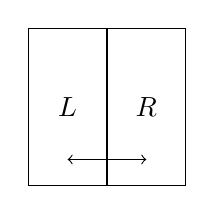
\begin{tikzpicture}
        \pgfmathsetmacro{\side}{1};
        \draw[] (0,0) -- (0, 2*\side) -- (2*\side, 2*\side) -- (2*\side, 0) -- cycle;
        \draw[] (\side,0) -- (\side, 2*\side);
        \draw (\side/2, \side) node[]{$L$};
        \draw (3*\side/2, \side) node[]{$R$};
        \draw[<->] (\side- \side/2, \side/3) --node[above]{$\De$} (\side + \side/2, \side/3);
    \end{tikzpicture}
\end{center}
Where $\ket{L}$ indicates that the particle is on the left half and $\ket{R}$ indicates that the particle is on the right half. The tunneling Hamiltonian becomes,
\[ H = - \De \br{\ket{L} \bra{R} + \ket{R}\bra{L}} \]
The parity operator takes $\ket{L}$ to $\ket{R}$ and vice versa. As a matrix,
\[ H = \begin{pmatrix}
    0 & - \De \\
    - \De & 0
\end{pmatrix} \qquad E_{\pm} = \pm \De \]
The energy eigenstates are,
\begin{align*}
E_- &= - \De \implies \ket{S} = \f{1}{\sqrt 2} \br{\ket L + \ket R} \\
E_+ &= + \De \implies \ket{A} = \f{1}{\sqrt 2} \br{\ket L - \ket R}
\end{align*}
As a demonstration of $H \ket{S} \propto \ket{S}$,
\begin{align*}
H \ket S
&= - \De \br{\ket L \bra R + \ket R \bra L} \f{1}{\sqrt 2}\br{\ket L + \ket R}  \\
&= - \f{\De}{\sqrt 2} \br{\ket L \cancelto{0}{\braket R L} + \ket R \braket L L +\ket R \cancelto{0}{\braket L R}+\ket L \braket R R}   \\
&= - \f{\De}{\sqrt 2} \br{\ket R + \ket L} \\
&= - \De \ket S
\end{align*}
Since $\pi \ket L = \ket R$ and $\pi \ket R = \ket L$,
\begin{align*}
    \pi \ket S & = \ket S\\
    \pi \ket A & = -\ket A
\end{align*}
If we were to set $\De= 0$, (i.e. prevent the possibility of tunneling) then we have that $E_+$ and $E_-$ become $0$. Then eigenstates are $\ket L$ and $\ket R$ which are not parity eigenstates. \\

\subsection{Parity Selection Rules}

Suppose we have two parity eigenstates $\ket \al$ and $\ket \be$.
\begin{align*}
    \pi \ket \al &= \ep_\al \ket \al \\
    \pi \ket \be &= \ep_\be \ket \be
\end{align*}
Where $\ep_\al, \ep_\be = \pm 1$. We can not look at the matrix elements of $\ve x$,
\[ \bra \be \ve x \ket \al = \bra \be \pi^{-1} \pi \ve x \pi^{-1} \pi \ket \al \]
But we know that $\pi$ is unitary and Hermitian,
\[ \bra \be \ve x \ket \al = \bra \be \pi^{\dagger} \pi \ve x \pi^{\dagger} \pi \ket \al \]
Or we can also right,
\[ \bra \be \ve x \ket \al = \bra \be \pi^{\dagger} \pi^{\dagger} \ve x \pi \pi \ket \al \]
But $\ket \al$ and $\ket \be$ are eigenstates of $\pi$.
\[ \bra \be \ve x \ket \al = \ep_\al \ep_\be \bra \be \pi^{\dagger} \ve x \pi \ket \al \]
Moreover $\pi^{\dagger} \ve x \pi = -\ve x$ by definition,
\[ \bra \be \ve x \ket \al = - \ep_\al \ep_\be \bra \be \ve x \ket \al \]
Therefore we have one of two cases:
\begin{enumerate}
    \item $\ep_\al \ep_\be = - 1$: one of the states is parity-odd while the other one is parity-even
    \item $\bra \be \ve x \ket \al = 0$: matrix elements of parity-odd operators can only be non-zero between states of different parity
\end{enumerate}

\subsection{Symmetries of Discrete Translations}

Heretofore we have talked about continuous symmetries like the symmetries of translations. Alternatively we can have symmetries associated with discrete translations. These symmetries arise all the time in condensed matter when considering the translations of a crystal lattice. \\

As a foundational example, consider a 1D periodic potential.

\begin{center}
    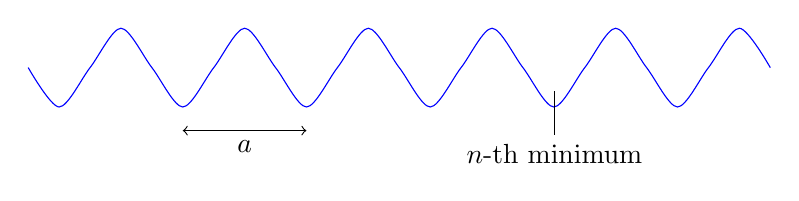
\begin{tikzpicture}
        % \draw[scale=0.5,domain=-3*pi:3*pi,smooth,variable=\x,blue] plot ({\x},{sin(deg(3*\x))});
        \draw[scale=0.5,domain=-3*pi:3*pi,smooth, variable=\x,blue] plot ({\x},{sin(deg(6*\x))});
        \draw[<->] (-3 + 0.25, -0.8) -- node[below]{$a$} (-3+ 0.25 + pi/2, -0.8);
        \draw[] (1.97, -0.8-0.05) node[below]{$n$-th minimum} -- (1.97, -0.8+0.5);
    \end{tikzpicture}
\end{center}

Where $V\br{x + a} = V\br{x}$. We have symmetry of translations by $a$ or any integer multiple of $a$. Therefore,
\[ T^{\dagger}\br{a}T^{\dagger} = V\br{x + a} = V\br{x} \]
We also have that $T^{\dagger}\br{a} \f{\ve p^2}{2m} T\br{a}$ so that $T\br{a} H = H T\br{a}$.
\[ \bs{H, T\br{a}} = 0 \]
We can find eigenstates of $H$ which are also eigenstate of $T\br{a}$. We will look at the limit of infinite barrier height; the particle has to be stuck in any of the minimal of the potential. Let $\ket n$ be the state in which the particle is in the $n$-th minimum.
\[ H\ket n = E_0 \ket n \]
And $T\br{a} \ket n = \ket {n+1}$ which implies that $\ket n$ is not an eigenstate of $T\br{a}$. Instead consider,
\[ \ket \te = \sum_{n = -\inf}^{\inf} e^{i n \te} \ket n \]
Since $\te \mapsto \te + 2 \pi m$, where $m$ is an integer does not change $e^{i n \te}$ (for all $ -\pi \leq \te \leq \pi$). The transition operator acting on $\ket \te$ is,
\begin{align*}
    T\br{a} \ket \te
    &= \sum_{n = - \inf}^{\inf} e^{i n \te} T\br{a} \ket n \\
    &= \sum_{n = - \inf}^{\inf} e^{i n \te} \ket {n+1} \\
    &= \sum_{n' - 1 = - \inf}^{\inf} e^{i \br{n' - 1} \te} \ket {n'} \\
    &= e^{-i\te}\sum_{n' = - \inf}^{\inf} e^{i n' \te} \ket {n'} \\
    &= e^{-i\te}\ket \te
\end{align*}
Therefore have that $T\br{a} \ket \te = e^{i \te} \ket \te$ is an eigenstate of $T\br{a}$ with eigenstate $e^{i \te}$. By linearity $\ket \te$ is \textit{also} and eigenstate of $H$.\\

To generalize this analysis assume that the barrier height is finite but large enough so that particles may only tunnel between nearest neighbor minimum. In this case our Hamiltonian will be very similar to the ``left/right'' tunneling amplitude discussed earlier. The matrix elements of $H$ for this system are $\bra{+1} H \ket{n}$. We assign to them the probability $- \De$ to be the probability amplitude for tunneling between nearest neighbor minima. We also assume define that $\ket n$ be an eigenstate $\bra n H \ket n = E_0$. Therefore,
\[H\br{n} = E_0 \ket n - \De \ket {n+1} - \De \ket{n-1} \]
Which means that $H$ acting on the translation eigenstate $\ket \te  = \sum_n = e^{i n \te} \ket n$ becomes,
\begin{align*}
H\ket \te
&= \sum_{n=-\inf}^{\inf} e^{i n \te} H \ket n \\
&= \sum_{n=-\inf}^{\inf} e^{i n \te} \br{E_0 \ket n - \De \ket {n+1} - \De \ket{n-1}} \\
&= \sum_{n=-\inf}^{\inf} e^{i n \te} E_0 \ket n - \sum_{n=-\inf}^{\inf} e^{i n \te} \De \ket {n+1} - \sum_{n=-\inf}^{\inf} e^{i n \te} \De \ket{n-1}
\end{align*}
\end{document}
